% \documentclass{aastex}
\documentclass[iop,tighten]{emulateapj}
\usepackage[utf8]{inputenc}
\usepackage{apjfonts}
\usepackage{multirow}

\usepackage{graphicx}
\usepackage{epstopdf}

\newcommand{\myshorttitle}{Wide-Field Near-IR Imaging of M31}
\newcommand{\myshortauthors}{Sick et al.}

\usepackage{color}
\usepackage[dvipsnames]{xcolor}
\usepackage[pdfauthor={\myshortauthors},pdftitle={\myshorttitle},colorlinks=true,citecolor=blue,linkcolor=blue,urlcolor=blue]{hyperref}
\usepackage{url}

\usepackage{amssymb}
\usepackage{amsmath}

\usepackage{natbib}
\bibliographystyle{apj}

\newcommand{\ie}{\textit{i.e.,~}}
\newcommand{\eg}{\textit{e.g.,~}}
\newcommand{\etal}{et~al~}
\newcommand{\vect}[1]{\boldsymbol{#1}} % vectors or images
\newcommand{\sw}[1]{\textit{#1}} % style software titles
\newcommand{\sn}{\ensuremath{S/N}} % signal to noise
\newcommand{\sersic}{S\'{e}rsic}
\newcommand{\iiwione}{\sw{`I`iwi 1.0}}
\newcommand{\androids}{\textsc{androids}}
\newcommand{\changeit}[1]{\textcolor{BrickRed}{\underline{#1}}} % markup bad sections
\newcommand{\todo}[1]{\textcolor{BurntOrange}{\textsf{#1}}} % markup TODOs
\newcommand{\mycomment}[1]{\textcolor{OliveGreen}{\textit{#1}}} % markup TODOs
\newcommand{\Fig}[1]{Fig.~\ref{fig:#1}}  % figure reference macro
\newcommand{\Eq}[1]{Eq.~\ref{eq:#1}}  % equation reference macro
\newcommand{\Tab}[1]{Table~\ref{tab:#1}}  % table reference macro
\newcommand{\Sec}[1]{\S\ref{sec:#1}}  % section reference macro

% To track draft versions in git
% \IfFileExists{vc.tex}{\input{vc}}{}

% aastex setup
\shorttitle{\myshorttitle}
\shortauthors{\myshortauthors}

\begin{document}
    % \IfFileExists{vc.tex}{\slugcomment{Version \VCRevision\ by \VCAuthor\ on \VCDateTEX , \VCTime.}
% }{\slugcomment{Revision unknown.}}
\slugcomment{Submitted to AJ.}
% \title{ANDROIDS I. New Insights in Wide-Field Near-IR Surface Photometry\\ with the Andromeda Galaxy (M31)}
\title{Andromeda (M31) Optical and Infrared Disk Survey \sc{i}.\\ New Insights in Wide-Field Near-IR Surface Photometry}
\author{Jonathan Sick, Stéphane Courteau}
\affil{Department of Physics, Engineering Physics \& Astronomy, Queen's University, Kingston, Ontario, K7L 3N6 Canada}
\email{jsick@astro.queensu.ca}
\author{Jean-Charles Cuillandre}
\affil{Canada-France-Hawaii Telescope Corp., Kamuela, HI 96743, USA}
\author{Michael McDonald}
\affil{Kavli Institute for Astrophysics and Space Research, MIT, Cambridge, MA 02139, USA}
\author{Roelof de Jong}
\affil{Astrophysikalisches Institut Potsdam (AIP), An der Sternwarte 16, 14482 Potsdam, Germany}
\and
\author{R. Brent Tully}
\affil{Institute for Astronomy, University of Hawaii, 2680 Woodlawn Drive, Honolulu, HI, USA}

% ============================================================================
\begin{abstract}
We present wide-field near-infrared $J$ and $K_s$ images of the Andromeda Galaxy (M31) taken with WIRCam at the Canada-France-Hawaii Telescope (CFHT) as part of the Andromeda Optical and Infrared Disk Survey (\androids).
This data set allows simultaneous observations of resolved stars and near-infrared (NIR) surface brightness across M31's \emph{entire} bulge and disk (within $R=22$~kpc), permitting a direct test of the stellar composition of near-infrared light in a nearby galaxy.
% Our survey complements the similar Panchromatic Hubble Andromeda Treasury survey by covering M31's entire disk, rather than a single quadrant, at similar wavelengths, albeit with lower spatial resolution.
Here we develop NIR observation and reduction methods to recover a uniform surface brightness map across the $3\arcdeg \times 1\arcdeg$ disk of M31 with 27 WIRCam fields.
Two sky-target nodding strategies are tested, and we find that strictly minimizing sky sampling latency does not enhance background subtraction accuracy, which is at best 2\% of the background level.
We fully describe our WIRCam reduction pipeline and advocate using flats built from night sky images over a single night, rather than dome flats that do not capture the WIRCam gain structure.
Contamination from scattered light and thermal background in sky flats has a negligible effect on the surface brightness shape compared to stochastic differences in background shape between sky and galaxy disk fields, which are on the order of 0.3\% of the background level.
The most dramatic calibration step is the introduction of scalar sky offsets to each image that optimizes surface brightness continuity.
This step reduces the mean surface brightness difference between observation blocks from 1\% to $<0.1$\% of the background level, though the absolute background level remains statistically uncertain to 0.15\% of the background level.
We present our WIRCam reduction pipeline and performance analysis here as a template for future near-infrared observers needing wide-area surface brightness maps with sky-target nodding, and give specific recommendations for improving photometry of all CFHT/WIRCam programs.
\end{abstract}
\keywords{methods: observational, techniques: photometric}
% ============================================================================
\section{Introduction}
\label{sec:intro}

Thanks largely to its proximity, kinship with the Milky Way, and being an ideal foil for modern galaxy formation models, the Andromeda Galaxy (M31) has been the focus of numerous investigations of galaxy structure \citep{Ibata:2005,Irwin:2005,McConnachie:2009,Courteau:2011} and stellar populations \citep{Williams:2002,Worthey:2005,Saglia:2010}.
The shapes, ages, kinematics and relative fraction of galaxy components (bulge, disk, halo) in large spiral galaxies like our own reveal precious information about their formation, accretion, and merging histories \citep[\eg see the review of][]{Kormendy:2004}.

Unfortunately, the fundamental task of disentangling galaxy components---which typically involves light profile decompositions, colour gradients and mass modelling---remains non-trivial.
Stellar population studies of spiral galaxies are thwarted by a three-fold degeneracy between stellar age ($A$), metallicity ($Z$) and ISM dust that can only be lifted by combining, at the very least, optical and infrared images with realistic dust models \citep{de-Jong:1996b,MacArthur:2004,Pforr:2012}.
Likewise, mass models of spiral galaxies suffer a degeneracy between the stellar $M/L$ and dark halo parameters that requires, in addition to an extended rotation curve, deep and accurate multi-band imaging to uniquely constrain the stellar $M/L$ ratio \citep{Dutton:2005,Courteau:2013}. 

Compounding these challenges are fundamental uncertainties in modern stellar population synthesis, particularly uncertainties in the interpretation of near-infrared (NIR) light.
For instance, optical-NIR SEDs yield unreliable population synthesis fits compared to optical-only SED fits.
This failure is largely attributable to inadequate stellar population synthesis recipes for NIR bands and naive parameterization of star formation histories \citep{Taylor:2011,Courteau:2013}.

First, spectral energy distribution (SED) fitting often relies on simplistic star formation history (SFH) parameterizations.
Because NIR colours lift age-metallicity-dust degeneracies, modelling of NIR bands may require additional sophistication, namely composite star formation and metal enrichment histories.
The appropriate form of SFH models cannot be constrained from the integrated light of galaxies alone (as is typically attempted); resolved colour-magnitude diagrams (CMDs) are both more effective and, in fact, essential at deriving non-parametric stellar population histories. 

Second, the NIR light is dominated by thermally-pulsating AGB (TP-AGB) stars from intermediate-aged stellar populations.
Modelling TP-AGB stars is most challenging due to their complex dredge-up cycles that change surface chemistry and temperature (the M- to C-type transition), and circumstellar winds that further perturb an AGB star's location in the CMD.
A proper calibration of NIR stellar population synthesis models \cite[\eg][Charlot \& Bruzual in prep.]{Maraston:2005} will yield a 30\%--50\% improvement in the estimation of stellar masses and ages of high redshift systems \citep[\eg][]{Maraston:2006,Bruzual:2007,Conroy:2010b,Conroy:2013}.

Our remedy for understanding both the structure of M31, and more fundamentally NIR stellar populations, is to survey the entire bulge and disk ($R \leq 22$~kpc) of M31 in both resolved and integrated stellar light at $J$ and $K_s$ wavelengths.
In doing so, we can directly relate a NIR stellar population's decomposition in the colour-magnitude plane to the panchromatic SED of M31.
Though such a calibration could be made with other galaxies, M31 is unique in its proximity so that even ground-based instrumentation can resolve its bright stellar population
For reference, $1\arcsec = 3.7~\mathrm{pc}$ across the disk of M31 \citep[we adopt $D_\mathrm{M31} = 785$~kpc,][]{McConnachie:2005}.

A wealth of photometric data exist for M31, however, none provide simultaneous observations of M31's resolved and integrated NIR light.
The best resource for resolved stellar populations across the entire disk of M31, to date, is the Local Group Galaxy survey \cite[LGGS,][]{Williams:2003,Massey:2006}.
This survey, although covering the $UBVRI$ wavelengths, does not extend to the $JHK$ NIR wavelengths most contentious for stellar population models.
Advancing our view of M31 to NIR wavelengths, \cite{Beaton:2007} assembled a 2.8\arcdeg\ $JHK_s$ mosaic of M31 with the 2MASS 6X program.
Those observations were also used by \cite{Athanassoula:2006} as evidence for a bar embedded in a classical bulge.
Beyond the bulge, the 2MASS 6X images have limited utility; background level uncertainties restrict their use to infer structural and photometric properties of the disk.
Further, the pixel scale of 1\arcsec\ and integration depth of 46.8 seconds prevent point source measurements of M31 stars in the 2MASS 6X images.
As a result, the then state-of-the-art NIR view of M31 is the 3.6 $\mu$m Spitzer/IRAC map of \cite{Barmby:2006}.
While Spitzer reduces uncertainties in background estimation, the pixel scale of 0\farcs86 prevents point source measurements of individual stars in the M31 disk.

Decompositions of M31's stellar populations have been made with high-resolution Hubble Space Telescope (HST) observations \citep{Brown:2003,Brown:2006,Brown:2008}.
These authors detected an intermediate age population in the inner halo of M31, and even disentangled debris associated with the Giant Stream around M31 in six fields sampling the outer disk, halo, and Giant Stream around M31 \citep{Brown:2009a}.
Similarly, though in the near-infrared, \cite{Olsen:2006} derived star formation histories within $22\farcs5\times22\farcs5$ fields in M31's inner disk and bulge with ground-based adaptive optics observations with the Gemini ALTAIR/NIRI instrument.
However these pencil beam surveys cannot be construed as representative of the entire Andromeda Galaxy.
Thus the boldest step forward in understanding M31's stellar populations is coming from the Panchromatic Hubble Andromeda Treasury Survey \citep[PHAT,][]{Dalcanton:2012}.
PHAT provides wide-field coverage from M31's centre to the $10$~kpc star forming ring, a panchromatic view of stellar populations from 3000\AA--17000\AA, and resolution of stars in very crowded environments such as the bulge.
Note that PHAT only covers a single quadrant of M31 making any global conclusions about M31's stellar populations incomplete.
Further, the wavelength coverage of HST/WF3 falls short of the $2.2$~$\mu$m $K$-band, making empirical calibration of the common NIR bands used by wide-field NIR surveys ($JHK$) impossible.
Thus there is good cause, even in the era of PHAT, to revisit M31 with a ground-based survey that covers the entire disk of M31 at NIR wavelengths, while using the best natural seeing in the northern hemisphere (on Mauna Kea) to resolve stars even more effectively than the previous ground-based survey of M31's disk (LGGS).

We present such a survey, the first instalment of the Andromeda Optical and Infrared Disk Survey (\androids), in this paper.
ANDROIDS uses the WIRCam instrument \citep{Puget:2004} on the Canada-France-Hawaii Telescope (CFHT), which is among the first generation of wide-field ground-based NIR detector arrays, covering a $21\farcm 5 \times 21\farcm 5$ field of view.
Indeed, the advent of detectors such as WIRCam makes such a wide-field, high-resolution survey of an object as vast as M31 possible.
The excellent natural seeing (0\farcs 65) on Mauna Kea is sufficient for resolving giant-branch stars throughout the disk of M31.

Recovering the true NIR surface brightness map of M31 is, however, technically challenging.
The NIR background (from both atmospheric fluorescence and instrumental thermal emission) is $\sim 10^3\times$ brighter than the NIR surface brightness of M31 at $R=20$~kpc, demanding exceptional background characterization.
Whereas most NIR galaxy surveys can measure the instantaneous background from blank sky pixels surrounding the galaxy on a detector array, M31's extended size requires physically nodding of the telescope away from the galaxy by 1\arcdeg--3\arcdeg\ to sample blank sky (called Sky-Target, or ST, nodding).
That we can never observe the instantaneous background on the disk of M31, but rather sample the sky at both a different location and time, introduces additional complications.
\cite{Adams:1996} clearly showed, with $9\arcdeg \times 9\arcdeg$ movies of the sky, that NIR sky emission has coherent spatial structure that moves across the sky over those scales, akin to a cirrus cloud system.
This assures that background sampled from a sky field \emph{will not} correspond directly to the sky affecting disk observations.

Besides background level, another concern is the accuracy of the surface brightness shape across individual WIRCam fields of view.
Spatial structures in the NIR sky can leave residual shapes in background subtracted disk images that ultimately affect our ability to produce a seamless NIR mosaic of M31.
\cite{Vaduvescu:2004} also found that detector systems themselves, in their case the (now decommissioned) CFHT-IR camera, can add a time-varying background signal whose strength may be comparable to the NIR surface brightness of the outer M31 disk.

Because such a large mosaic has never before been assembled in a ST nodding WIRCam program, we focus this contribution on engineering the best practices for this type of observing.
This includes: finding the optimal ST nodding cadence, defining the appropriate data reduction procedures for a WIRCam surface brightness reduction, and finally presenting an analysis of the surface brightness accuracy in wide-field WIRCam mosaics.

Section~\ref{sec:Observations} describes the novel observational strategies used to reduce background subtraction uncertainties.
Section~\ref{sec:reduction} presents the image reduction pipeline; with night sky flat fielding and median background subrtaction in Section~\ref{sec:flats}, and zero-point calibration practises in Section~\ref{sec:photocal}.
The accuracy of our WIRCam image calibrations are analyzed in Section~\ref{sec:flatanalysis}.
In Section~\ref{sec:scalar} we present our method for recovering the galaxy surface brightness by minimizing image-to-image differences across the mosaic, while in Section~\ref{sec:scalaranalysis} we analyze the results of this algorithm.
We estimate the systematic uncertainties in our mosaic solution in Section~\ref{sec:systematics}, where we also compare our technique to the Montage package \citep{Berriman:2008} and the Spitzer/IRAC mosaics.
Finally in Section~\ref{sec:conclusions} we summarize the uncertainty of NIR background subtraction on the scale of M31 and outline our ideal observation and reduction method.
In a future instalment we use resolved star counts to establish the NIR surface brightness of the M31 disk beyond $R > 15$~kpc.

\section{Observations}
\label{sec:Observations}

\begin{figure}[t]
\centering
\includegraphics[width=\columnwidth]{figs/fieldmap_colour}
\caption{\androids\ WIRCam field positions on M31.
Central blue fields are the 27 disk fields observed in 2007B, surrounded by 4 sky fields (blue with solid black outlines).
Red fields at center are the 12 disk fields observed in 2009B.
The red ring of 53 fields is the 2009B sky sampling ring.
The dashed yellow ellipse marks the M31 disk at $R=20$ kpc along the major axis.
Coordinates are centered on the nucleus of M31 with North up, and East is left.}
\label{fig:fieldmap}
% skysubpub/chart.py
\end{figure}

% Surface brightness CI from skyoffset/net_sky_level.py
% Median and 95% C.I.
% 2007B J 15.1195176911 ; 14.9139114767 -- 15.3477818651
% 2009B J dim 14.5613758489 ; 14.2933487068 -- 14.8544020768
% 2009B J bright 15.2006801085 ; 15.1336648803 -- 15.2789519627
% 2007B Ks 13.354737759 ; 13.1811645305 -- 13.6149313145
% 2009B Ks 13.27306929 ; 13.1173594814 -- 13.4222534742

\begin{table*}[t]
\caption[Summary of WIRCam observing programs]{Summary of WIRCam observing programs.
$N_\mathrm{disk}$ is the number of WIRCam fields covering the M31 disk in each semester (see \Fig{fieldmap}).
ST Nods with superscripts denote the number of times an observation is repeated for a given field.
$T_\mathrm{int}$ is the total integration time per disk field while $T_\mathrm{exp}$ is the integration time per WIRCam exposure.
\emph{Eff.} is the observing efficiency, or percentage of time in a program allocated to integrating the disk of M31, compared to nodding, read out and sky overheads.
$\mu_\mathrm{bkg}$ gives the range (min-max) of background surface brightnesses seen in each band.
PSF reports the distribution seeing as measured from the full width at half maximum (FWHM) of stellar point spread functions in the uncrowded sky images.}
\label{tab:obssummary}
    
    \centering
    \begin{tabular}{lllllllllll}
        & & & & $\frac{T_\mathrm{int}}{\mathrm{field}}$ & $T_\mathrm{exp}$ & Eff. & $\mu_\mathrm{bkg}$ & \multicolumn{3}{c}{PSF FWHM (arcsec)} \\ \cline{9-11}
    Semester & Band & $N_\mathrm{disk}$ & ST Nods & (min) &  (s) &  (\%) & (mag/arcsec$^2$) & 25th  & 50th & 75th \\
    \hline
    \multirow{2}{*}{2007B} & $J$ & \multirow{2}{*}{27} & [S$^3$T$^8$]$^{2}$S$^3$ & 12.5 & 47 & 49 & (15.4, 16.7) & 0.68 & 0.75 & 0.84 \\
     & $K_s$ &  & [S$^5$T$^{13}$]${^2}$S$^5$ & 10.8 & 25 & 42 & (13.4, 14.2) & 0.60 &  0.65 & 0.73 \\
     \hline
     \multirow{2}{*}{2009B} & $J$ & \multirow{2}{*}{12} & \multirow{2}{*}{[ST$^2$]$^{20}$S} & \multirow{2}{*}{13.3} & \multirow{2}{*}{20} & \multirow{2}{*}{26} & (15.0, 16.5) & 0.61 & 0.69 & 0.83 \\
                            & $K_s$ & & & & & & (13.4, 14.3) & 0.60 & 0.66 & 0.76 \\
    \end{tabular}
\end{table*}

M31 was observed in the NIR using the WIRCam instrument, mounted to the 3.6-meter Canada-France-Hawaii Telescope (CFHT), at the summit of Mauna Kea in Hawaii over multiple runs between 2007 and 2009.
Observations were carried out in the NIR $J$ ($\lambda_0 \sim 1.2 \mu\mathrm{m}$) and $K_s$ ($\lambda_0 \sim 2.2 \mu\mathrm{m}$) bands.

WIRCam is an array of four HgCdTe HAWAII-RG2 detectors \citep{Puget:2004}.
Each detector comprises $2048\times 2048$ pixels, with a scale of 0\farcs 3~pix$^{-1}$, which critically samples CFHT's typical seeing of 0\farcs 65.
WIRCam's detectors are arranged in a $2\times 2$ grid with 45\arcsec~gaps, so that the entire instrument covers $21.5\arcmin \times 21.5\arcmin$ of sky.
It is truly the advent of NIR focal plane arrays, like WIRCam, that has enabled wide-field studies of M31 in the NIR.

The \androids\ WIRCam survey is designed to simultaneously resolve stars and recover the integrated surface brightness of the entire M31 disk.
As discussed in \Sec{intro}, NIR observations require frequent monitoring of the background.
\cite{Vaduvescu:2004} found, for example, that the NIR background intensity can vary by 0.5\% per minute; yet the low surface brightness of M31's NIR disk at $R=20$~kpc requires the background level to be constrained to approximately 0.01\% \todo{(EXPRESS IN MAGS TOO)}.
With a $190\arcmin \times 60\arcmin$ optical disk, M31 is much larger than the WIRCam fields of view, and monitoring of the background zero-point is only possible by periodically pointing the telescope away from M31 towards blank sky through \emph{sky-target} (ST) nodding. 
The fundamental compromise of ST nodding observation programs is to balance the cadence of sky sampling with the efficiency of observing the target itself.
Although studies such as \cite{Vaduvescu:2004}, and references therein, provide good guidelines for NIR background behaviour, no program has attempted to construct a near-IR surface brightness mosaic covering an area as large and faint as M31's disk.

We now have the opportunity to experiment with different ST nodding strategies since observations were taken over the 2007B and 2009B semesters.
An objective of this study is to determine how observational design can improve the construction of a wide-field NIR mosaic by comparing the performance of two pre-defined observing strategies.

\begin{figure}[t]
\centering
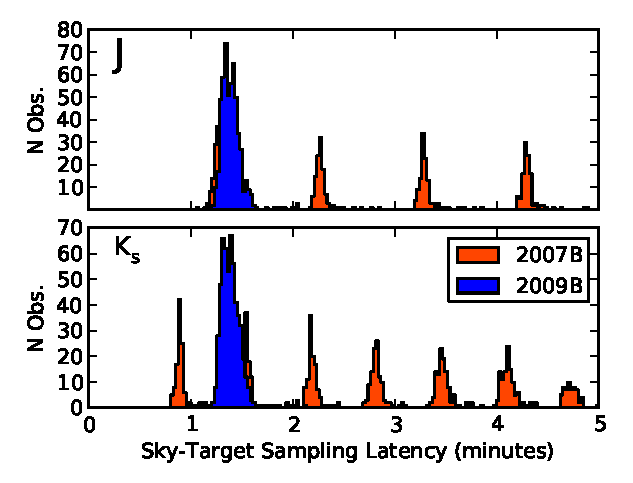
\includegraphics[width=\columnwidth]{figs/sky_target_lag}
\caption{Time latency between target observations and sky field sampling in the 2007B and 2009B WIRCam observing runs.
The 2009B program was designed to ensure that no disk sample would be removed by more than 1.5 minutes from a sky sample by using a STTS nodding pattern.}
\label{fig:sky_target_lag}
% made with skysubpub/obs_run_stats.py
\end{figure}

\begin{figure}[t]
\centering
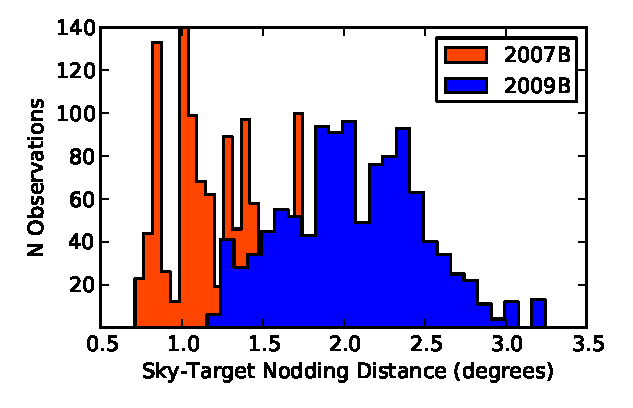
\includegraphics[width=\columnwidth]{figs/sky_target_dist}
\caption{Distance between sky and target observations in the 2007B and 2009B WIRCam observing runs.
The larger nodding distance of 2009B is a consequence of sky ring sampling.
The maximum nodding distance across the sky ring was purposely set to $\sim 3$\arcdeg\ to avoid excessive time overheads (see \Fig{fieldmap}).
As such, a given disk field only samples roughly half of the full sky ring.}
\label{fig:sky_target_dist}
% made with skysubpub/obs_run_stats.py
\end{figure}

\begin{figure}[t]
\centering
\includegraphics[width=\columnwidth]{figs/sky_level_hist}
\caption{Background levels observed in the 2007B and 2009B programs, as applied to each target field.}
\label{fig:net_sky_level}
% made with skyoffset/net_sky_level.py
\end{figure}

\subsection{2007B Semester}
\label{sec:obs7}

The initial survey was carried out in the 2007B semester by the CFHT Queue Service Observing under photometric conditions.
Here M31 is covered with 27 contiguous WIRCam fields out to the optical radius where $\mu_V=23$ mag arcsec$^{-2}$ at $R=20$~kpc.
The fields are arranged with at least 1\arcmin\ overlap in declination, and approximately 5\arcmin\ overlap in right ascension.
The field configuration is shown in \Fig{fieldmap}.

As shown in Table~\ref{tab:obssummary}, each field was integrated for $16\times 47~\mathrm{s} = 12.5$ minutes in $J$ and $26\times 25~\mathrm{s} = 10.8$ minutes in $K_s$.
These integrations are sufficiently deep for resolved stellar photometry to reach at least 1~mag below the tip of the red giant branch, a crucial requirement for decomposing the contributions of red giant and asymptotic giant branch stars to the NIR light.

The 2007B ST nodding strategy was motivated by a canonical understanding of NIR background behaviour, since ST nodding background subtraction had never been attempted on this scale before.
The NIR background intensity can be expected to change by 5\% in 10~minutes \citep{Adams:1996,Vaduvescu:2004}.
Since the background itself is $\sim10^3\times$ brighter than the outer disk of M31 in the NIR, a 5\% uncertainty in the background would be fatal to our objective of recovering M31's extended NIR surface brightness.
To constrain background brightness within 1\%, we ensured that a sky sample would be no more than 5 minutes removed from a M31 target image.
Given the respective exposure times (chosen so as not to saturate with the background flux), this implied a sky ($S$)--target ($T$) observing sequence of $S^3T^8S^3$ in $J$ and $S^5T^{13}S^5$ in $K_s$.\footnote{Superscripts here denote the number of times an observation is repeated in sequence for a given target disk field.}
Four sky fields were chosen (\Fig{fieldmap}), and each disk field was associated with a single sky field.

\subsection{2009B Semester}
\label{sub:obs9}

Analysis of the 2007B data revealed that the adopted sky-target nodding strategy was not sufficient for recovering the M31 surface brightnesses due to uncertainties in the background.
Repeatedly sampling one of only four sky fields also proved not ideal.
This motivated the 2009B observing campaign.

Rather than replicate the 28-field footprint of the 2007B campaign, we observed 12 new fields in 2009B (see red boxes in \Fig{fieldmap}) that overlap each other and all of the 2007B footprints, to form a network of well-subtracted fields.
Thus the 2009B observations augment and calibrate the 2007B NIR mapping.

To improve background subtraction fidelity, we recognized challenges not fully appreciated in the 2007B survey design.
Not only does the background change rapidly in time, it possess a significant spatial structure on the scale of WIRCam fields and larger.
This has two ramifications: the background level sampled at a sky field \emph{will not} necessarily reflect the background present at the disk, and that the background in each WIRCam frame has a 2D shape, not simply a scalar level.

This resulted in three principle changes to the observing strategy. First, we chose to minimize latency between sky and target observations with a ST$^2$S pattern. That is, each target observation was directly paired with a sky observation taken within 1.5 minutes (\Fig{sky_target_lag}).

Second, we also increased the number of repetitions on each field, so that each field is observed 40 times in each band in a [ST$^2$]$^{20}$S pattern. This repetition enables averaging over spatial sky background structures on the scale of WIRCam fields.

Finally, we employ a pseudo-randomized sky-target nodding pattern where no sky field is used repeatedly for a disk field.
In order to maintain rapid telescope nods, only northern sky fields serviced the northern disk, and similarly for the southern fields; the maximum offset on the sky was 3\arcdeg\ (see \Fig{sky_target_dist}).
This non-repetitive sampling of sky fields yielded two possible advantages: 1) when a median background image is constructed, many \emph{background shapes} are combined, possibly yielding an intrinsically flatter background image (see \Sec{mediansky}), and 2) if there is a coherent structure in the NIR background, sampling sky fields degrees apart in rapid succession should average out these systematic biases in estimating the background level \emph{on the galaxy disk}.

\section{Image Preparation}
\label{sec:reduction}

\begin{figure*}[t]
\centering
\includegraphics[width=\textwidth]{figs/pipeline_flowchart}
\caption{Flowchart representation of the \androids\ WIRCam pipeline, from receipt of CFHT \iiwione\ data products to rendering of M31 mosaics.
\todo{Label article sections within the flowchart (once known).}}
\label{fig:flowchart}
% made with Illustrator
\end{figure*}

While CFHT distributes calibrated WIRCam data products, we haven chosen to replace much of their data reduction recipes with our own to optimize and explore the limitations of wide-field NIR surface brightness maps.
An overview of the pipeline is shown in \Fig{flowchart}; the principle steps are 1) astrometry, 2) source masking, 3) night sky flat fielding, 4) zero-point estimation against 2MASS sources, 5) median sky frame construction, 6) image calibration with zero-points and median sky subtraction and 7) background optimization and mosaic production in three hierarchical steps.

\subsection{Choice of Starting Point}

CFHT offers WIRCam data in two degrees of preprocessing with the \iiwione\ pipeline: an image that has been corrected for nonlinearity, dark subtracted and flat fielded (\texttt{*s.fits}); and an image that has been background subtracted, in addition to all the previous treatments (\texttt{*p.fits}).
In order to implement our own calibration strategy, our mosaics stem from \texttt{*s.fits} products (though we note that \texttt{*p.fits} products are still used for astrometry and source masking, see below).
Nonetheless, two \iiwione\ processing stages included in \texttt{*s.fits} products must be handled carefully.

\paragraph{Cross-talk correction} WIRCam integrations prior to March 2008 (includes the 2007B data set, not the 2009B data) suffered from electronic cross talk within the detector.
This cross talk is manifested in repeating rings above and below saturated stars.\footnote{See \url{http://cfht.hawaii.edu/Instruments/Imaging/WIRCam/WIRCamCrosstalks.html}.}
By default, the \iiwione\ pipeline removes this cross talk by subtracting a median of the 32 amplifier slices.
Unfortunately, this algorithm fails in cases where the background has a surface brightness gradient (such as on the disk of M31) and produces a brightness gradient that is stronger than the galaxy surface brightness itself.
Loic Albert (then at CFHT) kindly re-processed our 2007B data set with the cross-talk correction omitted.

\paragraph{Flat fielding} A pecularity of \texttt{*s.fits} images is that even though they are flat fielded using dome flats as CFHT, those products still exhibit strong non-uniformity, dust artifacts and surface defects.
% From CFHT website on Dome Flats
% We are using dome flats obtained at the beginning of each observing run on the observatory dome illuminated with a tungsten lamp. We obtain a cube of 15 raw flats with the dome light turned on and subtract the 15 raw flats of the same exposure time with the light turned off. This ensures any instrumental thermal component is removed. We typically use 5-6 second exposure times for wide band filters and up to 30 second exposure times for narrow band filters and target fluxes of about 10000 adu on lamp-on flats.
%
% Here is how dome flats are processed:
%
% Each detector is treated entirely independantly.
% All raw flats (lamp on and off) are multiplied by the bad pixel mask, subtracted by their corresponding dark, and the background level is measured using a simple median.
% Flat-off. Some flat-off images are rejected when their background level is different by more than 1% compared to the others, or when more than 3 sigma off the others. Then the flat-off images are normalized to 1, a cube is created and the median (through dimension 3) is obtained. Finally, the median flat-off image is multiplied back by the median of all initial background levels.
% Flat-on. Each flat-on has the final flat-off subtracted from it. Then the same rejection criteria as for flat-off images are used. Then all flat-on images are normalized to one before being put in a cube. Finally, the median of the cube is obtained (through the third dimension). This produces the final processed dome flat image.
% Flat fields show mostly a radially increasing flux level and, fortunately, no high spatial frequency fringes. The pixel to pixel quantum efficieciency variations are of the order of a few percents.
We note that CFHT produces dome flats (for each queue run) from median stacks of 15 images taken under a tungsten lamp, subtracted from images of the same integration time taken with the lamp off.
This procedure should remove the additive thermal background from the flat, ensuring that the flat field is a purely multiplicative calibration.
Despite this, the presence of dust artifacts betrays the fact that dome flats do not reproduce the same illumination pattern as sky photons.
Similarly, the presence of surface defects in dome-calibrated images could be caused by disparities in both the optical path and the colour of the tungsten lamp versus the night sky background.
In this work, we find that WIRCam images can be adequately flat fielded using night sky flats.
We give a visual demonstration of the superiority of night sky flat fielding in \Fig{flattenedimage_comparison}: surface defects left by dome flat fielding are removed with night sky flat fielding.

One interesting feature of \texttt{*s.fits} images is the appearance of horizontal banding corresponding to the 32 amplifiers that service independent horizontal bands of each WIRCam detector (seen in \Fig{flattenedimage_comparison}).
It is odd that a dome flat failed to calibrate such electronic structures in a detector, and one might expect that the such banding should be calibrated with an additive correction.
Indeed, this banding is absent of fully-processed \iiwione\ images due to median sky frame \textit{subtraction}.
However, we maintain that the flat fielding is the correct treatment for these structures since they appear to be proportional to the skyglow background throughout the night (which can vary by 10\% during a night), yet are still corrected with a single night sky flat.

Our \androids\ pipeline thus begins with \texttt{*s.fits} data that have been \textit{uncorrected} for dome flat fielding.
That is, we multiply the \texttt{*s.fits} image with its associated dome flat.\footnote{Dome and twilight flats are made available by CFHT, \url{http://limu.cfht.hawaii.edu:80/detrend/wircam/}.}
The result is an image that retains \iiwione's prescription for dark subtraction, bad pixel masking and non-linearity correction, ready for our own sky flat fielding (to be described in \Sec{flats}).

\subsection{Astrometry}

Early in the pipeline we build a unified astrometric frame for our image set using \sw{SCAMP} \citep{Bertin:2006}.
\sw{SCAMP} matches stars in \sw{Source Extractor} \citep{Bertin:1996} catalogs of each WIRCam frame both internally (to $\sigma_\mathrm{int}=0\farcs 10$), and against the 2MASS Point Source Catalog \citep{Skrutskie:2006} to a precision of $\sigma_\mathrm{ref}=0 \farcs 15$.
% Values obtained from Scamp XML output
By processing all 4286 frames in the \androids /WIRCam survey simultaneously, \sw{SCAMP} allows an accurate and internally consistent coordinate frame for our mosaic.
\sw{SCAMP} handles this data volume gracefully provided we cull the input star catalogs for stars with $S/N > 100$, and by using the \texttt{SAME\_CRVAL} astrometry assumption that the WIRCam focal plane geometry is stable.
Also note that we build our \sw{Source Extractor} catalogs using the fully-processed \texttt{*p.fits} \iiwione\ images since those are adequate for source detection and astrometry.
While \sw{SCAMP} is capable of also fitting a photometric solution for each frame, we choose to establish photometric zero-points later in our pipeline using a combination of background flux observed across the detector array, and bootstrapping against 2MASS sources observed in uncrowded 2MASS images.

\subsection{Non-Sky Pixel Masking}

A second preliminary pipeline stage is source masking.
For each sky image we build masks that yield only blank pixels to aid with background level estimation, sky flat construction (\Sec{flats}) and median sky frame construction (\Sec{mediansky}).
These masks are built by a combination of \sw{Source Extractor} object maps (detected in \texttt{*p.fits} images) and hand-drawn polygon regions that cover the diffraction spikes and halos of very bright foreground stars.
These masks, along with the \iiwione\ bad pixel mask, are combined with \sw{WeightWatcher} \citep{Marmo:2008}.

\begin{figure}[t]
\centering
\includegraphics[width=\columnwidth]{figs/flattenedimage_comparison}
\caption{Comparison of a WIRCam frame cutout processed with dome flats by the \iiwione\ pipeline (top), and with sky flats (bottom).
Both images are shown in linear counts with identical level ranges.
No median background subtraction has been applied.
Dome flats leave WIRCam images with dust artifacts (left) and detector surface defects (right). Furthermore, the 64-pixel high horizontal amplifier bands are clearly visible.
Simply using sky flats eliminates these artifacts.
}
\label{fig:flattenedimage_comparison}
% skysubpub/flattened_image_comparison.py
\end{figure}

% \begin{figure}[t]
% \centering
% \includegraphics[width=3.5in]{figs/flatratio_09BQ01_Ks}
% \caption{Difference image between the 09BQ01 $K_s$ (queue run) sky flat and the \texttt{domeflat\_8302B\_20090728HST143302\_Ks} dome flat used in the \iiwione\ pipeline, in percent.
% Using the median night sky illumination over a WIRCam queue run, rather than a dome lamp, results not only in $>2$\% edge-to-edge difference in the large scale WIRCam illumination function, but also in different characterizations of gain structure in the WIRCam detector amplifiers (the 32 horizontal bands in each of the four WIRCam detectors).}
% \label{fig:domeflatratio}
% % made with wircam/skyflat/plot/flatratio.py
% \end{figure}

\section{Sky Flat Fielding and Median Sky Subtraction}
\label{sec:flats}

As we mentioned previously in \Sec{reduction}, dome flats fail to properly calibrate dust, amplifier gain and surface defects in WIRCam data (see \Fig{flattenedimage_comparison}).
Sky flats are an appropriate alternative, both because of the abundant background photons (any NIR imaging program can use its own images to build sky flats), and because sky flats directly match the illumination path and colour of observations.
Sky flats also have the advantage of being contemporaneous with observations: if the WIRCam flat field is variable, then sky flats can be built to track such variability.
This is a distinct advantage over dome flats, which CFHT builds at the beginning of every WIRCam queue run, or even twilight flats that can only be built once per night.

Despite these advantages, sky flats are built on the assumption that all background illumination in a night sky image is proportional to the flat field function.
Several contaminants prevent this from being true: thermal emission from the detector or telescope structures, can add a significant background in the $K_s$ band, and scattered light (\eg off the camera's cold pupil stop) and further perturb the proportionality of flat field images.
Ideally one would subtract these contaminants from images before constructing sky flats.
Then science images could be flat fielded, and additive contaminants in science images would be automatically removed in subsequence median background subtraction.
Note that both dome flats and twilight flat fields can distinguish additive contaminants from the multiplicative flat field function.
Dome flats are built from the differences of images taken with the lamp on and off, directly removing any thermal component from the flat field.
% TODO describe what dome flats can do. Are they immune to the cold stop? No, dome does not. Twilight might.
Twilight flats can also treat additive contamination by capturing images at different levels of sky illumination so that linear fits to each pixel allow any additive bias to be removed.
In the case of sky flat fielding, however, we \emph{cannot} disentangle additive from multiplicative processes in images.
We must assume that additive contaminants are negligible, and simply divide images by the median sky shape.
In the following sections, we test this assumption to verify that sky flats are the ideal tool for calibrating WIRCam images.

A second assumption built into sky flat construction is that sky glow is uniform across the detector.
Wide-field images of the near-infrared night sky show that sky glow has rich spatial and temporal variations.
However, by marginalizing over a large number of sky images, any illumination bias in the sky can be mitigated.
The 2009B observing program even took this marginalization process further by sampling pseudo-random sites on the sky while building sky flats. One degree of control that can be exerted over sky flat construction is the time window that sky images are drawn from.
Using a wide window, the length of a queue observing run, asserts confidence that the intrinsic WIRCam flat field function is stable over several days, while producing the statistically flattest residual sky illumination pattern.
Shorter windows make the opposite assertion that the WIRCam flat field is stable, and that any bias in sky shapes can be tolerated.

We investigate three sky flat designs in this study, labelled \texttt{QRUN}, \texttt{NIGHT} and \texttt{FW100K}.
\texttt{QRUN} flats are built from all sky integrations taken during a queue run, and through a given filter.
For the \androids\ program, 25--637 (typically $\sim 140$) sky images, obtained over a sequence of a $\leq 10$ days, are composed into a \texttt{QRUN} flat.
\texttt{NIGHT} flats are from all sky integration taken during a single night, through a given filter.
Because observations are observed in queue service observing mode, the ensemble of sky images typically sample 0.5--3 hours of a night.
Last, we introduce \emph{real-time} sky flats that are rapidly updated throughout the night in case the WIRCam illumination function and gain structure is unstable.
\texttt{FW100K}, is designed such that the pool of sky images reaches cumulative background levels of at least 100,000 ADU, or that the time span from first to last sky integration is no longer than two hours.
Given the 07B $J$-band ST nodding pattern, 15 sky integrations are accumulated in 50 minute windows, whereas the more frequent nodding in the 09B campaign shortened this window to 20 minutes (though as long as 50--90 minutes in dark sky conditions).
The brighter $K_s$ sky calls for just 7--13 integrations in 07B, or 10--20 integrations in the 09B campaign.
This number of $K_s$ sky samples was accumulated within 10--30 minutes in 07B, or 10--70 minutes in 09B.

\subsection{Implementation of Sky Flat Fielding and Median Background Subtraction}
\label{sec:flatbuilding}

We now describe the technical details of sky flat fielding and median background subtraction steps.
Recall from \Fig{flowchart} that the inputs of flat field construction are `de-flattened' images that retain the linearity and dark-current subtraction of the \iiwione\ pipeline.

\subsubsection{Sky Flat Construction}
\label{sec:skyflatconstruction}

According to the type of sky flat being constructed, \texttt{QRUN}, \texttt{NIGHT} and \texttt{FW100K}, ensembles of sky images are formed.
Given an ensemble of sky integrations, our next task is to scale the intensity of each image.
This scaling obeys three requirements: 1) each image frame in the median stack is at the same level, 2) each WIRCam detector has a unified zero-point, and 3) the sky flat across the whole array is flux normalized.\footnote{It is also acceptable to establish chip-to-chip zero-point offsets using differential 2MASS photometry, rather than from background surface brightness. In \Sec{detector_zp} we establish the equivalence of the two methods.}
This scaling is determined by the median pixel level measured on each detector for each sky integration---let us denote these median levels as $\alpha_{i,j}$ for the $i$th sky image's level in detector $j$, $j=1, 2, 3, 4$.
To avoid bias in the background estimate, we mask any pixels that do not sample blank sky.
\sw{Source Extractor} \citep{Bertin:1996} is used to define stars and background galaxies (we use \iiwione\ \texttt{*p.fits} images to detect and mask sources), while hand-drawn polygon regions cover diffraction spikes and the diffuse halos around bright galactic stars. These masks, along with the \iiwione\ bad pixel mask, are combined with \sw{WeightWatcher} \citep{Marmo:2008}.

From the ensemble of images produced by an individual WIRCam detector, we compute the median background level: $\beta_j = \mathrm{median}(\alpha_{1,j}, \alpha_{2,j}\ldots \alpha_{n,j} )$.
Further, we also compute $S$, the median of all median detector levels: $S=\mathrm{median}(\beta_j)$.
Then each sky image is scaled by the factor $f_{ij} = \beta_j / (\alpha_{ij} S)$.
Note that the factor $\alpha_{ij}^{-1}$ normalizes each image to the same level for stacking, while the ratio $\beta_j / S$ adjusts the level of each detector according to detector-to-detector zero-point offsets.
% Indeed, detector-to-detector zero-point offsets can be measured as $-2.5 \log_{10}(\beta_i / \beta_1)$, as shown in \Fig{fw100k_zpdiff}.
% WIRCam detector \#1 (North-West quadrant) is clearly the most sensitive, while the dispersion indicates the level of gain variability in WIRCam.
% We also note systematic differences in spectral response of WIRCam detectors in the $J$ and $K_s$ of order 5\%.
% 0.05 mag is about 4.5%

The flat itself is built by median combination.
Median combination of a stack of hundreds of $2048\times2048$ pixel images, each with a weightmap masking astronomical sources, is computationally intensive.
A convenient solution is to use \sw{Swarp} \citep[an image-mosaicing software package,][]{Bertin:2002} in a mode that combines images pixel-to-pixel.
Once the sky flat is built, it is divided from the appropriate science images to produce a flat-fielded data set.

\subsubsection{Median background subtraction}
\label{sec:mediansky}

Since M31 is much larger than individual WIRCam fields, background is subtracted (to first order) using the background levels found in contemporary sky images.
Section~\ref{sec:Observations} described the sky-target nodding sequences chosen for the 2007B and 2009B observing campaigns. 
Although a scalar background level can be estimated from a sky image, and subtracted from the paired target images, it is common to construct a median background image, the same size as the WIRCam frames, and subtract this 2D image from target images.

Independent median background images for each WIRCam detector are produced by choosing a sky image (the primary sky image) and four other sky images taken at adjacent times.
Across each image, the median background intensity is recorded.
A Source Extractor object mask, as used in \Sec{flatbuilding} for flat fielding, removes bias from astrophysical sources.
Each sky image is \emph{additively} scaled to a common intensity level, allowing differences in overall background amplitude to be ignored by the median combination.
As described in \Sec{flatbuilding}, \sw{Swarp} is used to median-combine the sky images with non-sky pixel masks.
Since the background has only low-frequency spatial information, these median background images are smoothed with a Gaussian kernel (note this is quite different from the function of median background images applied to dome-flat processed WIRCam data, where median background subtraction also removed pixel-to-pixel artifacts).
This median background image is then additively scaled back to the original level of the primary sky image.

Each science image is background subtracted by first identifying the median background frame whose primary image was taken most closely in time.
That paired median background frame is subtracted from the image.

\section{Photometric calibration}
\label{sec:photocal}

Our flat field procedure necessitates a revision of photometric zero-points.
Since our program is observed in short ($\sim 1$ hour) blocks in CFHT's queue service observing, we do not have the necessary airmass baseline to solve for nightly zero-point and atmospheric extinction terms for each band.
Instead, we estimate photometric zero-points by directly bootstrapping against sources from the Two Micron All Sky Survey (2MASS) Point Source Catalog (PSC) \citep{Skrutskie:2006}.
Although these are not standards, the ensemble of 2MASS stars may be treated as such.
Since the disk of M31 is crowded, and 2MASS has low resolution ($1\arcsec$~pix$^{-1}$), we choose to directly estimate zero-points only in the sky images.
We estimate the zeropoints of disk images from a sliding window average of zeropoints from adjacent sky images (analogous to the median background subtraction procedure, described in \Sec{mediansky}).

Specifically, instrumental photometry of stars in the uncrowded sky fields is obtained with Source Extractor \citep{Bertin:1996}.
We use the \texttt{AUTO} photometry mode to capture the full stellar light without using aperture corrections.
2MASS PSC objects are matched to our Source Extractor detections by position using J. Sick's \sw{Mo'Astro}\footnote{\url{http://moastro.jonathansick.ca}} Python package, that manages the full 2MASS PSC in a MongoDB database.
The 2MASS PSC contains many galaxies, and many 2MASS sources are saturated in our deeper WIRCam images.
Thus we select sources with $J < 14$ or $K_s < 15$ magnitudes, and FWHM $<1$\arcsec according to our Source Extractor photometry.
Additionally, we select sources with $J-K_s < 0.8$ (typical of foreground Milky Way stars) as we observe larger zero-point residuals in redder stars.
After filtering, typically 200 matched 2MASS sources remain in typical WIRCam images.
Given a joined catalog of 2MASS and instrumental photometry (in ADU) in a specific sky image, we estimate an instrumental zero-point as the median photometric offset:

\begin{equation}
  \label{eq:photcal}
  m_0 = \langle m_\mathrm{2MASS} + 2.5 \log_{10}(\mathrm{ADU}/T_\mathrm{exp}) \rangle.
\end{equation}

Our data show no trend in zero-point vs $J-K_s$ color index.
Hence, following practice at CFHT, we do not apply a color transformation between 2MASS and WIRCam bandpasses.
Internal testing at CFHT with synthetic photometry indicates that colour transformation coefficients may be $A_J = 0.05$ and $A_{K_s}=-0.005$ (K. Thanjuvar, priv.\ comm.)
For typical M31 RGB stars with $J-K_s\sim 1$, this colour transformation would be a $< 0.1$~mag effect.

Given that 2MASS stars in each image have photometric uncertainties $0.05 \lesssim \sigma_{\mathrm{2MASS~mag}} \lesssim 0.3$, the typical statistical zero-point uncertainty, $\sigma_{m_0}$, is 0.1~mag in a single image.
However, the random uncertainty of zero-points adopted from sliding window averages across multiple sky images are $<0.01$~mag.
% see $andpipe/wircam/calibset/photcal/singleimg/uncertainty_dists.py for photometry properties 

\section{Analysis of Sky Flat Fielding and Background Subtraction Methods}
\label{sec:flatanalysis}

Near-infrared sky flat fields are fraught with \emph{additive} contaminants from thermal emission and scattered light.
Although we regard a perfect near-infrared flat field as unattainable, we can test which flat field prescription (\texttt{QRUN}, \texttt{NIGHT} or \texttt{FW100K}) performs best, and assess whether the final quality of our NIR M31 mosaics are limited by uncertainties from flat fielding or from ST-nodding background subtraction uncertainties.


\subsection{Evolution of Real Time Sky Flats}
\label{sec:flatevo}

% \begin{figure*}[t]
% \centering
% \includegraphics[width=\textwidth]{figs/fw100k/fw100k_movie}
% \caption{Spatio-temporal evolution of \texttt{FW100K} sky flats, shown as percent difference of the flat fields 15, 30, 60 and 90 minutes after the initial sky flat of the night.
% Sky flat evolution on three nights is shown: (a) 2009B $K_s$ observing block with the telescope staring at a sky field, (b) 2009B $K_s$ observing block with regular sky-target nodding, and (c) a 2007B observing block with sky-target nodding.}
% \label{fig:fw100k_movie}
% % made with andpipe/wircam/skyflat/plot/flatratio.py
% \end{figure*}
\begin{figure*}[t]
\centering
\includegraphics[width=\textwidth]{figs/55136_Ks_fw100k_night_grid}
\caption{
Evolution of \texttt{FW100K} $K_s$-band sky flats over the course of three hours.
Percent difference maps of \texttt{FW100K} sky flats relative to the \texttt{NIGHT} sky flat are shown in the upper grid (time evolves left to right, from the top row).
Colors in the percent difference maps show $\pm2\%$ variation.
The bottom panels show the background level observed in each detector as a function of time.
The bottom panel shows zero-point differences computed for each \texttt{FW100K} sky flat as a function of time since the first \texttt{FW100K} flat between detector \#1 and detectors \#2, 3 and 4 respectively.
}
\label{fig:fw100k_movie}
% made with andpipe/wircam/skyflat/plot/flatratio.py
\end{figure*}

% \begin{figure}[t]
% \centering
% \includegraphics[width=\columnwidth]{figs/fw100k/fw100k_globalamp_timeseries_55136_Ks}
% \caption{Time evolution of the mean flat field level of amplifier bands in the four WIRCam detectors in \texttt{FW100K} sky flats made over three hours.
% Amplifier bands are colour-coded according to their order on the array: red lines at the bottom, green in the middle, and blue at the top.
% Although the levels of individual amplifiers differ by 10\%, their order is consistent, indicating that amplifier gain is extremely stable.
% The jitter is due to detector-to-detector zero-point normalization (\Sec{flatbuilding}) uncertainty, or measurement biases.}
% \label{fig:fw100k_globalamp_timeseries_55136_Ks}
% % wircam/skyflat/plots/amp_level_global.py
% \end{figure}

A key advantage of sky flats is their close temporal correspondence to the data.
Taken to the extreme, our \texttt{FW100K} flats are updated with sliding windows of approximately 30~minutes.
Here we investigate the nature of evolution in the `real-time' \texttt{FW100K} flats throughout a night.
% In doing so, we can assess whether sky flat evolution is driven by proportional effects, or additive contamination such as a thermal background or scattered light.
In \Fig{fw100k_movie} we show the evolution of \texttt{FW100K} sky flats relative to a single \texttt{NIGHT} sky flat over the course of three hours on a single night.
This observing sequence, unlike the typical observing patterns, consisted of consecutive integrations on sky fields, without nodding to the M31 disk, so that an uninterrupted view of sky flat evolution could be visualized.
Over the course of three hours, we see a large-scale shape perturbation move across the detectors from left to right.
On the same timescale, the background \emph{level} has changed by as much as 30\% (\Fig{fw100k_movie} middle panel).

Although \Fig{fw100k_movie} clearly demonstrates that real-time \texttt{FW100K} sky flats evolve smoothly, it does not distinguish whether the evolution is driven by proportional effects or by additive contamination such as a thermal background or scattered light.
However, we do note that the patterns are similar to those observed in the CFHT-IR by \cite{Vaduvescu:2004}, who report a thermal background contamination.

% In \Fig{fw100k_movie} we show percent difference images between \texttt{FW100K} sky flats made at intervals of 15, 30, 60 and 90 minutes after an initial sky flat.
% After just 30~minutes, the shape of the \texttt{FW100K} skyflats deviates by 0.5\% from the initial flat field shape.
% By 60 minutes, the deviation exceeds 1\%.
% Evidently, our WIRCam skyflats are stable on timescales less than 30 minutes---much less than a queue run.

% Nonetheless, the spatio-temporal evolution takes many forms.
% In some cases (\Fig{fw100k_movie}b) the flat field deviations are axisymmetric, while in others there is a distinct East-West pattern (\Fig{fw100k_movie}ac).
% We interpret these as instabilities in the WIRCam illumination function on the scale of minutes.

An alternative interpretation is that these sky flat deviations are instabilities in the WIRCam detector electronics.
The dominant macroscopic electronic feature in WIRCam flat fields are the amplifier bands.
Each WIRCam detector is divided into 32 horizontal bands (each 64 pixels high) that are read out into independent amplifiers.
These amplifiers have gains that result in levels that differ by 10\% in flat field images.
However, we find that the gain of each amplifier band is stable throughout the night, at a level of $<0.1\%$ relative to other amplifiers.
Thus sky flat evolution is not driven by WIRCam gain instabilities, but by large scale variations in the flat field function or an additive background component.

\subsection{Detector-to-Detector zero-point Evolution}
\label{sec:detector_zp}

\begin{figure}[t]
\centering
\includegraphics[width=\columnwidth]{figs/fw100k/fw100k_betadiff}
\caption{Distribution of real-time sky flat scaling factors, measuring detector-to-detector zero-point differences relative to detector \#1 (red: \#2, green: \#3, blue: \#4) in $J$ and $K_s$ bands.
}
\label{fig:fw100k_zpdiff}
% $andpipe/wircam/skyflat/plot/chip_zp_diff.py
\end{figure}

\begin{figure}[t]
\centering
\includegraphics[width=\columnwidth]{figs/fw100k/fw100k_chip_to_chip}
\caption{Distribution of mean detector-to-detector zero-point offsets for sky images processed by real-time sky flats.
Zero-point offsets between detectors \#1 \& \#2, \#1 \& \#3, and \#1 \& \#4 are plotted as
red, green and blue histograms, respectively, for the $J$-band (top) and $K_s$-band (bottom).}
\label{fig:fw100k_chip_to_chip}
% andpipe/wircam/calibset/photcal/singleimg/chip_consistency_zp_fixa.py
\end{figure}

We can test if real-time sky flats are tracking evolution in the intrinsic WIRCam flat field function, or merely a background contamination, by examining the detector-to-detector photometric consistency against 2MASS standard photometry.
Recall that our sky flats are designed to unify the zero-points of the four WIRCam detectors by scaling according to the modal background levels seen in each detector.
Any additive background contamination will introduce detector-to-detector zeropoint offsets.
In \Fig{fw100k_zpdiff} we examine zero-point differences implied by the modal background values in real-time \texttt{FW100K} sky flats, which are computed as $-2.5 \log_{10}(\beta_i / \beta_1)$ from the discussion in \Sec{skyflatconstruction}.
From \Fig{fw100k_zpdiff} we see that the estimated zero-point differences between detectors can be variable over a range of 0.05~mag in the $K_s$-band.
This variability is more prominent in $K_s$-band sky flats than in $J$-band.

We can test the validity of these zero-point transformations by verifying the photometric zero-points of individual detectors against 2MASS stars, as was done in \Sec{photocal}.
Figure~\ref{fig:fw100k_chip_to_chip} shows the distribution of mean detector-to-detector zero-point offsets observed in images processed by \texttt{FW100K} sky flats.
We find that zero-points are consistent within $\pm 0.1$ mag, though we detect a small possible systematic bias between detectors \#1 and \#4 at the level of $0.03$~mag.
The origin of the this zero-point bias can be seen in the bottom panel of \Fig{fw100k_movie}, which tracks the detector-to-detector zero-point evolution estimated from each real-time \texttt{FW100K} sky flat over the course of 3~hours.
The relative zero-points slowly shift by $\lesssim 0.05$~mag in concert with the evolution in the shapes of \texttt{FW100K} sky flats due to time-varying additive contamination (upper panel of \Fig{fw100k_movie}).
These results confirm that our sky flats \emph{are} contaminated by a thermal background, albeit at a small level.
The systematic photometric bias at the level of $0.03$~mag is negligible compared to the photometric uncertainty of individual stars.

\subsection{Frame residuals shapes}
\label{sec:frameblockresiduals}

We have established (\Sec{flatevo}--\Sec{detector_zp}) the presence of an additive contamination in WIRCam sky flats that varies over the course of a night and has a slight ($<0.1$~mag) influence on photometric calibration.
Here we demonstrate how contamination in sky flats influences our observations of M31's surface brightness by examining the residual shapes of individual frames against the median shape of the disk (as assembled in our wide-field mosaic, \Sec{scalar}).
This also provides a test of the timescale on which the intrinsic WIRCam flat field function is stable.
If the residuals of datasets treated by \texttt{QRUN} or \texttt{NIGHT} sky flats vary systematically with time, in correspondence with the results of \Sec{flatevo}, then the flat field function of WIRCam truly would be variable throughout a night.
In this case, \texttt{FW100K} sky flats should be most appropriate.
This effect should be exacerbated in signal- (not sky-) dominated fields as flat field errors grow in proportion to signal strength.

Our 2009B observations of field M31-37 in the $K_s$ band are ideal for this experiment: a single detector in that field covers the core of M31, and observations were taken into two blocks, covering a total window of 2~hours (most blocks for this program are observed by the CFHT queue in a half hour).
Both the high surface brightness and wide time baseline in this field should highlight flat field bias and variation.
Figures~\ref{fig:frame_residuals_M31-37_Ks_fw100k_medsky}--\ref{fig:frame_residuals_M31-37_Ks_QRUN} we show the residual shapes of individual WIRCam frames against the median shape of the mosaic, given \texttt{FW100K}, \texttt{NIGHT} and \texttt{QRUN} sky flattening, respectively, in field M31-37 in the $K_s$ band.
% That is, we produce difference images between each WIRCam frame and the block mosaic.
To analyze the shapes of these difference images we marginalize the difference images along rows (left side of \Fig{frame_residuals_M31-37_Ks_fw100k_medsky}), and columns (right side of \Fig{frame_residuals_M31-37_Ks_fw100k_medsky}).
Note that these marginalizations are done for each detector in the $2\times2$ WIRCam array; the core of M31 resides in detector \#2 (lower-right).
In that high surface brightness region, there are strong surface brightness residuals that clearly point out flaws in the flat field itself.

Comparing Figures~\ref{fig:frame_residuals_M31-37_Ks_fw100k_medsky},~\ref{fig:frame_residuals_M31-37_Ks_nightset}~and~\ref{fig:frame_residuals_M31-37_Ks_QRUN}, we see that both \texttt{FW100K} and \texttt{NIGHT} sky flats have similar performance, where frames vary in surface brightness $\pm 0.5\%$ at the core of M31.
The exception are \texttt{QRUN}-treated frames that show an evolution on the order of $\pm 1\%$ of the $K_s$-band sky brightness over a similar time scale as indicated in \Fig{fw100k_movie}.
This indicates that \texttt{QRUN} sky flats, which are built over several nights of data, are unsuitable for capturing the WIRCam flat field function.
While this indicates that the intrinsic WIRCam flat field function varies detectably from night-to-night, the performance equivalence of \texttt{FW100K} and \texttt{NIGHT} sky flats indicates that the WIRCam flat \emph{does not} vary throughout the night.
% Again, we conclude that spatial variability tracked by the \texttt{FW100K} sky flats, and visualized in \Fig{fw100k_movie}, must reflect additive contamination (thermal background or scattered light) that can easily vary throughout the night.

It is useful to contrast the frame shape residuals seen in detector \#2 with those in other detectors, where the disk surface brightness is lower.
There, both \texttt{FW100K} (\Fig{frame_residuals_M31-37_Ks_fw100k_medsky}) and \texttt{QRUN} (\Fig{frame_residuals_M31-37_Ks_QRUN}) show similar residual distributions, on the order of $\lesssim 0.2$\% of the NIR background brightness.
Further, the results are not monotonically varying in time, as they are in detector \#2, and indeed appear to vary essentially randomly.
We interpret this frame residual behaviour as being caused by random additive background processes, distinct from flat field biases that are proportional to surface brightness.
We extend this analysis across the entire data set below.

\begin{figure*}[p]
\centering
\includegraphics[width=\textwidth]{figs/frame_residuals/M31-37_Ks_fw100k_medsky}
\caption{Residual shapes of individual \texttt{FW100K} sky flat-processed WIRCam integrations of the M31 disk to the median (mosaic) shape for the field M31-37, $K_s$-band, observed in the 2009B semester.
Residuals have been marginalized across the $x$ (left) and ($y$) (right) axes to provide 1D views.
Axes match WIRCam's $2\times2$ detector footprint.
Individual integrations are coloured by their time after the first disk integration.
The centre of M31 is located in the lower-right detector (\#2); surface brightness bias in these regions betray the presence of flat field bias. Lower surface brightness regions are dominated by shape variations on the order of $\pm 0.2\%$ of background level, interpreted as additive uncertainties associated either with the detector, skyglow, or both.}
\label{fig:frame_residuals_M31-37_Ks_fw100k_medsky}
% made with wircam/shape/frame_block_residuals/plot_field_slices.py
\end{figure*}

\begin{figure*}[p]
\centering
\includegraphics[width=\textwidth]{figs/frame_residuals/M31-37_Ks_nightset_medsky}
\caption{Residual shapes of individual of the M31-37 $K_s$ field, processed with \texttt{NIGHT} sky flats.
Compared to \Fig{frame_residuals_M31-37_Ks_fw100k_medsky}, \texttt{NIGHT} sky flats capture reliable the shape in the signal-dominated detector \#2 as well, if not better, than \texttt{FW100K} flats.
The WIRCam flat field function is the stable over the course of a night.
}
\label{fig:frame_residuals_M31-37_Ks_nightset}
% made with wircam/shape/frame_block_residuals/plot_field_slices.py
\end{figure*}

\begin{figure*}[p]
\centering
\includegraphics[width=\textwidth]{figs/frame_residuals/M31-37_Ks_queuesky_medsky}
\caption{Residual shapes of individual of the M31-37 $K_s$ field, processed with \texttt{QRUN} sky flats.
Compared to Figs.~\ref{fig:frame_residuals_M31-37_Ks_fw100k_medsky} and~\ref{fig:frame_residuals_M31-37_Ks_nightset}, \texttt{QRUN} sky flats clearly do not capture flat field evolution that occurs over the course of 90-minutes, yielding systematically evolving realizations of bulge-dominated surface brightness in detector \#2 (lower-right). In the more sky-dominated regions of the image (detector \#4), \texttt{QRUN} sky flats produce images with similar stability to \texttt{FW100K} and \texttt{NIGHT} sky flats, indicating that the limit of additive uncertainties associated with sky or instrumental background variations is reached here.}
\label{fig:frame_residuals_M31-37_Ks_QRUN}
% made with wircam/shape/frame_block_residuals/plot_field_slices.py
\end{figure*}

\subsection{Distributions of frame shape residuals}
\label{sec:frameblockresidualhist}

\Fig{frame_diffs_skyfrac} shows the distribution of frame-block residual shape amplitudes, measured at the 95\% difference interval.
In essence, this measures the consistency of capture the shape of each M31 block.
As in our test of median sky frame flatness (\Sec{medianskyshapes}), we see that the consistency of frame shapes is $\sim 0.3\%$ of the background level.
This result is seen universally amongst the \texttt{QRUN}, \texttt{NIGHT}  and \texttt{FW100K} sky flat pipelines and for 2007B and 2009B observing schemes, agreeing with our observation in \Sec{frameblockresiduals} that in background dominated regimes (as most of our blocks are) frame shape consistency is \emph{not} correlated with flat field bias.
Rather, we interpret \Fig{frame_diffs_skyfrac} as measuring the amplitudes of \emph{additive} stochastic background shapes originating either from the sky, or associated with the instrumentation itself.
Effectively, \Fig{frame_diffs_skyfrac} illustrates the \emph{flatness limit} of WIRCam frames observed with large sky-target nods, sky flat fielding, and median sky subtraction.

\begin{figure}[t]
\centering
\includegraphics[width=\columnwidth]{figs/frame_residuals/framediffs_skyfrac_cdf}
\caption{Cumulative distributions of scalar difference amplitudes between individual frames and blocks in the $J$ (top) and $K_s$ (bottom) mosaics, measured as a dispersion of pixel differences at the 95\% level.
  Whether processed with \texttt{QRUN} (red), \texttt{NIGHT} (green) or \texttt{FW100K} (blue) sky flats, or observed in 2007B (solid lines) or 2009B (dotted lines), the residual amplitude differences between frames and blocks are similarly distributed.
The mean amplitude difference is $0.3\%$ of the $J$ background brightness ($0.2\%$ in $K_s$).
}
% Made with andpipe/wircam/shape/frame_block_residuals/plot_frame_residuals_hists.py
\label{fig:frame_diffs_skyfrac}
\end{figure}

% \mycomment{Note that shape variability appears uncorrelated with sky level or time since sunset (unlike sky level; see \texttt{python andpipe/wircam/skyanalysis/shapevar\_correlations.py}.
% There may be a correlation against airmass, but it is weak.}

\subsection{Shapes of Median Background Frames}
\label{sec:medianskyshapes}

Another test of sky flats is their ability to produce an unbiased sky background, up to the level of intrinsic sky variations.
This test can be made by examining the median background frames (\Sec{mediansky}) produced by \texttt{QRUN}, \texttt{NIGHT} and \texttt{FW100K}-processed data sets.
We measure the amplitude of shapes across the $10\arcmin \times 10\arcmin$ WIRCam frame as the 2-standard deviation interval (95\%) of each median sky image's pixel distribution: $2 \sigma(\mathrm{med~sky})$.
In \Fig{mediansky_amplitude} the cumulative distribution functions of the background shape amplitudes are presented for each set of flat fielded data, in each band and for each semester.

\texttt{QRUN} sky flats, which are known to be incorrect (\Sec{frameblockresiduals}), produce median backgrounds with the largest amplitudes---as much as 3\% of the background.
Compared to the other flats, the \texttt{QRUN} sky flats are biasing the background shape, relying upon the median background subtraction process to effectively flatten the sky background.
\texttt{FW100K} sky flats have the opposite effect.
The temporal windows from which \texttt{FW100K} sky flats are constructed are nearly the same span as that for median background images, so the background amplitude is unsurprisingly negative.
\texttt{FW100K} sky flats divide all structure in images, be they multiplicative or additive in origin.
\texttt{NIGHT} flats produce median backgrounds with moderate amplitudes, and, unlike the \texttt{FW100K} data set, these amplitudes are similar in both bandpasses.
The slightly larger background amplitude in the $K_s$-band \texttt{NIGHT} data set may reflect an additional thermal background observed beyond the sky glow observed in both bands.

A surprising result from \Fig{mediansky_amplitude} is that backgrounds in 2009B images are not flatter than in 2007B.
Recall that median sky images are composed of five sky frames taken closest to a disk frame.
In 2007B, all sky frames were sampled from the same coordinate on the sky and span a 12~minute window covering sky integrations taken before and after a disk image (for both $J$ and $K_s$ sky-target nods).
In 2009B, sky frames were sampled from randomly chosen sites along the sky field ring (\Fig{fieldmap}) with a window typically spanning 15 minutes.
Thus both 2007B and 2009B median sky images span similar time windows, although the 2009B strategy attempts to marginalize over five distinct sites  on the sky (and thus sky background shapes) while 2007B median sky images do not.
From \Fig{mediansky_amplitude} we conclude that this marginalization does not effectively occur, implying that the background shapes sampled from distinct sites on the sky \emph{are} correlated.
Since wide-field movies of the NIR sky \citep{Adams:1996} suggest that this should not be true, there much of the structure in the median background images is an instrumental background.
Similar backgrounds are seen by \cite{Vaduvescu:2004} in the CFHT-IR camera.

\begin{figure}[t]
\centering
\includegraphics[width=\columnwidth]{figs/mediansky_amplitude_cdf}
\caption{Cumulative distribution function of background level amplitudes across median sky images processed with \texttt{QRUN} (red), \texttt{NIGHT} (green) and \texttt{FW100K} (blue) sky flats for the $J$ (top) and $K_s$ (bottom) bands. Real-time (\texttt{FW100K}) sky flats produce much flatter median sky frames, with mean shape amplitudes of 0.3\% ($J$) to 0.1\% ($K_s$) of the NIR sky level, while the mean amplitude of \texttt{QRUN}-flat processed sky images is 1.5\% of the background level, and as high as 3\% of the background level. \texttt{NIGHT} flat-processed data generate mean shape amplitudes of $\sim 0.6\%$ of the background level.
}
\label{fig:mediansky_amplitude}
% made with $andpipe/wircam/shape/mediansky_amplitude.py
\end{figure}


\subsection{Section Summary}
\label{sec:shapeconclusions}

We have thus far described how individual WIRCam frames of the M31 disk are calibrated according to the pipeline outlined in \Fig{flowchart}.
In this section we have analyzed the performance of our flat field, median background subtract and photometric calibration prescriptions.
Here we summarize our findings on the accuracy of surface brightness shapes reproduced by WIRCam in a sky-target nodding observing program.

Night sky flat fields are preferable to dome flats because sky flats properly calibrate dust, detector surface, and gain structures thank to a proper illumination of the entrance pupil.
Such flats can be easily made from programme data.
Specifically, we advocate \texttt{NIGHT} flats, which are built from all sky images taken over a single night, because they capture night-to-night variations in the WIRCam flat field not captured by \texttt{QRUN} flats (compare Figs.~\ref{fig:frame_residuals_M31-37_Ks_nightset} and~\ref{fig:frame_residuals_M31-37_Ks_QRUN}).

Although we confirm that night sky flats are afflicted by an \emph{additive} contamination (\ie thermal background, or scattered light) that varies on sub-hour timescales (\Fig{fw100k_movie}), this contamination impacts the photometric zero-point at a level of $0.03$~mag. 
This \emph{does not} impact the overall surface brightness fidelity of our mosaic.
Since the \androids /WIRCam mosaic of M31 is almost entirely background dominated, we are principally limited by background subtraction, which is non-trivial since the background cannot be directly measured on the M31 disk given our current field of view.
Ultimately we find that the \emph{shape} of the background on the disk can be known to within 0.3\% of the NIR background levels (\Fig{frame_diffs_skyfrac}).
By comparison, the typical amplitude of median sky images is $\sim 0.6\%$ of both the $J$ and $K_s$ background levels.
Note that it is impossible for a NIR observing program with large ST nods to subtract background shapes better than the 0.3\% we find here: the shape of the background at the target will always be distinct from background shapes measured at designated sky fields.

To summarize, we have spent considerable effort demonstrating that \texttt{NIGHT} sky flats are appropriate for our application, and the impact of thermal background and scattered light on flat fields and zero-points are negligible compared to background uncertainties due to NIR sky glow.
In the following sections we assemble NIR mosaics of M31 using images processed according to the preceding sections, using \texttt{NIGHT} sky flats and show that the single most important calibration for wide-field NIR mosaicing is sky offset optimization.

\section{Sky Offset Optimization}
\label{sec:scalar}

\begin{figure}[t]
\centering
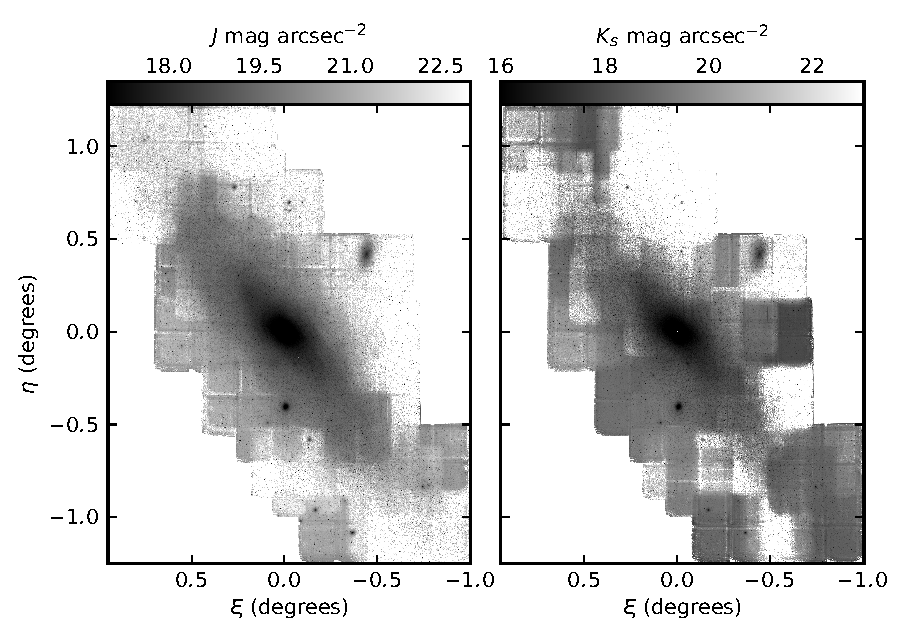
\includegraphics[width=3.5in]{figs/raw_mosaics}
\caption{Median background subtracted WIRCam $J$ (left) and $K_s$ (right) mosaics of M31 processed according to \Sec{reduction}--\Sec{photocal} using \texttt{NIGHT} sky flats.}
\label{fig:raw_mosaics}
% made with skysubpub/mosaic_plots.py
% + skysubpub/raw_mosaic.py
\end{figure}

In \Fig{raw_mosaics}, we plot mosaics (assembled using \sw{Swarp}) from \androids\ frames processed with the pipeline discussed in \Sec{reduction}--\Sec{photocal} and adopting the \texttt{NIGHT} sky flat prescription favored in \Sec{shapeconclusions}.
Although these image preparations can constrain the surface brightness \emph{shape} of a WIRCam frame by $\lesssim 0.3\%$ of the sky level, \Fig{raw_mosaics} demonstrates that the true level of the background on M31's disk is lost by the temporal and spatial of sky glow between disk and sky field observations.
This results in the distinct field-to-field surface brightness discontinuities seen in \Fig{raw_mosaics}.
However, we can use the constraint that all overlapping pairs of images composed in our mosaic should have equal surface brightness in their intersections.
To enforce this constraint, we solve for a \emph{sky offset} for each image: a small scalar nudge of intensity that can be added or subtracted from each image so that all images in the mosaic have continuous surface brightnesses.
Note that we use the term sky offset for these intensity adjustments, but in practise these offsets are agnostic of the cause of background subtraction error that they correct.
Since our mosaics are made from many inter-connected images (3924 $J$ and 4972 $K_s$ image frames), our optimization of sky offsets can provide powerful constraints on the true level of the background at the M31 disk.

\sw{Montage} is a FITS mosaicing package \citep{Berriman:2008} originally written for the 2MASS survey that includes sky offset estimation (background rectification, in their terminology) functionality.
\sw{Montage} can solve sky offsets either as scalar levels, or as planes.
Sky offsets are then chosen iteratively by looping through each image pair and choosing the offset needed to minimize the difference image of that pair, counting previous sky offset estimates.
Sky offsets are refined over several loops through the entire set of overlapping image pairs until convergence is reached (that is, once incremental adjustments to sky offsets diminish below user-specified threshold).
Although this iterative implementation of sky offset optimization is elegant, its accuracy has never been formally analyzed in literature, to our knowledge.
In particular, we are interested in the robustness of Montage sky offsets against local minima in the $N$-dimensional solution space of sky offsets, given a mosaic of $N$ independent images.
Further, the optimization is slow, given the several thousand frames in our mosaics.
Thus we decided to implement our own sky offset algorithm, although a comparison to the \sw{Montage} solution is given in \Sec{systematics}.

\subsection{Sky Offset Implementation}
\label{sec:msrnm_algo}

Our sky offset algorithm is based on two features that distinguish it from the \sw{Montage} implementation.
First, the optimization is carried out in three hierarchical stages to accommodate the large number of images.
Second, we use a downhill simplex algorithm \cite[][hereafter, NM]{Nelder:1965} with re-convergence checks rather than the iterative approach of the \sw{Montage} sky offset solver.
We begin with \texttt{NIGHT}-sky flat calibrated, median sky subtracted, and photometrically calibrated image set that are resampled using \sw{Swarp} to a common pixel in an Aitoff equal-area project with the native WIRCam pixel scale of 0\farcs 3~pix$^{-1}$.

We address the sky offset optimization hierarchically by considering the geometry of the WIRCam detectors in a $2 \times 2$ grid and arrangement of 39 WIRCam fields on the M31 disk (See \Fig{fieldmap}).
The first stage of optimization is to stack all \emph{detector frames} (images taken with a given detector, at a given field) into \emph{stacks}.
The offsets applied to WIRCam frames to build stacks are labelled $\Delta_F$.
Next, we solve for the offsets $\Delta_S$ ensure surface brightness continuity across the four stacks in a WIRCam field.
We call the combined unit of four stacks a \emph{block}.
The last stage of optimization solves for the offsets $\Delta_B$ applied to each block to ensure surface brightness continuity across the mosaic.
The net scalar sky offset applied to each frame is thus

\begin{equation}
  \Delta_\Sigma = \Delta_F + \Delta_S + \Delta_B.
  \label{eq:netoffset}
\end{equation}

\noindent After each stage of optimization, the scalar sky offsets are added to the WIRCam frames, stacks and blocks and Swarp is used to median co-add the images to generate stacks, blocks and a mosaic, respectively.
Using this hierarchical scheme ensures that at worst, the number of dimensions in our optimizations is 39, as opposed to the number of WIRCam frames (a factor $10^2$ reduction).

We use two algorithms for solving sky offsets.
Solving $\Delta_F$ offsets in the first stage is trivial since all frames simultaneously overlap.
Thus it is sufficient to simply compute a mean surface brightness across all frames, and directly compute offsets ($\Delta_F$) between between the levels of each frame and the mean level.
In the last two stages, stacks are blocks, respectively, are arranged in networks of overlapping pairs.
For this case we introduce our NM simplex-based offset optimization algorithm.

We identify overlaps between images in a brute-force fashion according to their frames in the mosaic pixel space, defined by the \texttt{CRPIX}, \texttt{NAXIS1} and \texttt{NAXIS2} header values of the resampled images.
For each overlapping image pair, we compute a difference image, and ultimately a median difference, $\langle \vect{I}_i - \vect{I}_j \rangle$.
While computing the median difference, we mask bad pixels using weight maps (propagated by \sw{Swarp}) and expand this mask with sigma clipping.
Along with a difference estimate, we also record the area $A_{ij}$ of unmasked pixels in the overlap, and the standard deviation of the difference, $\sigma_{ij}$.

We can estimate the optimal set of scalar sky offsets, $\Delta_i$, for each image $i$ by minimizing the objective function:

\begin{equation}
    \mathcal{F} \left(\Delta_1,\ldots,\Delta_n \right) = \sum_{i,j} \mathcal{W}_{ij} \left( \langle \vect{I}_i - \vect{I}_j \rangle - \Delta_i + \Delta_j \right)^2.
    \label{eq:objf}
\end{equation}

\noindent Note that each coupled image pair is its own term in the objective summation, and that there are as many degrees of freedom ($\Delta_i$) as there are images in the mosaic.
Each coupling is tempered by a weighting term $\mathcal{W}_{ij}$:

\begin{equation}
    \mathcal{W}_{ij} = \frac{A_{ij}}{\sigma_{ij}},
\end{equation}

\noindent so that more priority is given to couplings of larger areas ($A_{ij}$), and small standard deviations of their difference images ($\sigma_{ij}$).

The objective function in \Eq{objf} puts no constraint on the net sky offset: $\sum \Delta_i$.
Assuming that background subtraction errors are normally distributed, and not biased, sky subtraction offsets should not add a net amount of flux to the mosaic.
Fortunately, it is possible to impose this constraint \textit{post facto} by subtracting the mean offset from the sky offsets:

\begin{equation}
    \Delta_i^* = \Delta_i - n^{-1}\sum_{j=1}^n \Delta_j.
    \label{eq:netzero}
\end{equation}

\noindent In the limit that sky offsets $\Delta_i$ are drawn from a Gaussian distribution, with standard deviation $\sigma_\Delta$, the absolute brightness of the whole mosaic will be uncertain by $\sigma_\Delta / \sqrt{N_\mathrm{images}}$.
The consequences of this uncertainty are revisited in \Sec{systematics}.

Given the image coupling records, we optimize the set of $\Delta_i$ by applying the object function (\Eq{objf}) to NM downhill simplex algorithm.
The NM algorithm is naturally multi-dimensional and does not require knowledge of the gradient of the objective function.
Instead, the NM algorithm operates by constructing a geometric simplex of $N+1$ dimensions that samples the sky offset parameter space.
By evaluating the objective function at each vertex of the simplex, the NM algorithm adapts the simplex shape to ultimately contract upon a minimum.

The NM algorithm will converge into any local minimum without necessarily seeking the global minimum of the objective function.
We resolve this issue with two methods: ensuring re-convergence, and sampling different starting conditions.

The practice of ensuring reconvergence in a downhill optimization is suggested by \cite{Press:2007}.
Upon each convergence, the optimal point in the simplex, $\vect{p}$, is recorded.
A new simplex is then generated where one vertex is $\vect{p}$, and the rest are $\vect{p}+\vect{\delta}$ where $\vect{\delta}$ is a normal random variable of mean zero, and standard deviation $\sigma_\mathrm{restart}$.
That is, the simplex of the restart retains one vertex upon the previously found minimum, while the other vertices surround that minimum.
We set $\sigma_\mathrm{restart}$ to $2\times$ the dispersion of image-to-image differences.
Our optimization iterative converges and re-converges simplexes until the same minimum is consecutively arrived upon, indicating that the NM algorithm has arrived upon a robust solution.
Our sky offset optimizations for 39 blocks typically require $\sim1000$ restarts before converging definitively.

Besides ensuring reconvergence, we also start several independent NM simplex optimizations from random starting points in parameters space to seek a globally optimal sky offset solution.
We find that $N_s=50$, and possibly fewer, starts are quite sufficient for an optimization with 39 sky offset parameters (such as the fitting of $\Delta_B$ block offsets in mosaic).
For each start, an initial simplex is generated randomly.
Since each point in the $N$ by $N+1$ simplex is a suggested sky offset for a given field, each offset is randomly sampled from a normal distribution whose dispersion is $3\times$ the standard deviation of image-to-image differences to ensure parameter space is well covered.
Note that each simplex start and series of subsequent restarts can be performed in parallel.
Once all simplex runs are complete, the set of sky offsets belonging to the run that yielded the smallest value of the objective function is adopted.

\section{Analysis of Scalar Sky Offsets}
\label{sec:scalaranalysis}

Figure~\ref{fig:scalar_mosaics} presents the fruits of our WIRCam pipeline and sky offset optimization.
Compared to our mosaics without sky offsets, \Fig{raw_mosaics}, the sky offset optimization is clearly essential for assembling wide-field NIR mosaics.
These mosaics are not yet perfect; field-to-field discontinuities at a level of 0.05\% of background remain, and large-scale background residuals perturb the outer M31 disk.

\begin{figure}[t]
	\centering
		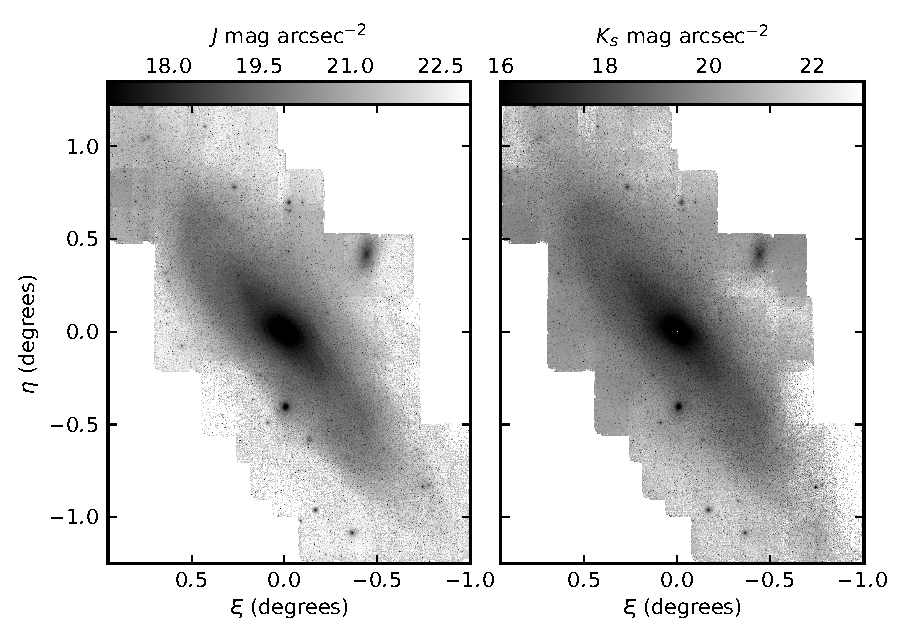
\includegraphics[width=3.5in]{figs/scalar_mosaics}
	\caption{Scalar-sky fitted WIRCam $J$ (left) and $K_s$ (right) mosaics of M31. Note the significant qualitative improvement compared to the original, median background-subtracted, images in \Fig{raw_mosaics}.}
	\label{fig:scalar_mosaics}
	% made with skysubpub/mosaic_plots.py
\end{figure}

\subsection{Amplitudes of Sky Offsets}
\label{sec:offset_amplitudes}

The distribution of scalar sky offsets provides an excellent characterization of background subtraction uncertainties when using sky-target nodding.
Recall that sky offsets are optimized hierarchically: WIRCam frames are fitted to stacks, stacks are fitted into blocks of four contemporaneously-observed WIRCam detector fields, and these blocks are fitted into a mosaic.
\Tab{offset_hierarchy} lists the standard deviations of these offset distributions with respect to the typical background level observed in the $J$ and $K_s$ bands.

% NOTE ON MEAN SKY LEVELS
% According to andpipe/wircam/calibset/mosaic/scalar_offset_hierarchy.py:
% Mean J Level: 894.19 muJy. Mean Ks Level: 19902.80 muJy
% But note that in WIRCam instrumental ADU/s, teh mean sky levels are:
% J: 122 ADU/s, Ks: 488 ADU/s. see $andpipe/wircam/skyanalysis/mean_sky_level.py

Note that the sky offsets, as a percentage of background level, are comparable in the $J$ and $K_s$ bands, despite the background being $\sim 4\times$ brighter in $K_s$ than $J$ (see \Fig{net_sky_level}).
This indicates that spatio-temporal variations in the NIR background are monochromatic.

Within the hierarchy of background fitting, simply fitting frames to a stack (with $\Delta_F$) is most significant: a correction on the order of 2\% of the background intensity.
Fitting blocks into a mosaic ($\Delta_B$) is a further $\sim 1$\% correction.
Overall, the temporal and spatial lags of sky-target nodding induce a 2\% uncertainty in the background level at the target.
It is this level of uncertainty that sky offset optimization must diminish to transform uncorrected mosaics (\Fig{raw_mosaics}) into ones that reproduce the disk with fidelity (\Fig{scalar_mosaics}).

Note that offsets to fit a stack into a block ($\Delta_S$) of four detector field stacks are smallest: 0.1\% of the background level.
This suggests that on the scale of the $2\times 2$ WIRCam array, the contemporaneously observed detector frames are subjected to nearly identical biases in background.
Stack offsets, then, arise from uncertainties in the pipeline's measurement of the background level from single frames in two stages: estimating detector-to-detector zero-point offsets from frame background levels (\Sec{skyflatconstruction}) and again when subtracting a median background frame (\Sec{mediansky}).
Indeed, in \Sec{flatanalysis} we show that median background images have shape amplitudes of 0.3\% of the background level and that individual frames have surface brightness shapes that are uncertainty at a level of 0.2\%; $\Delta_S$ sky offsets are thus a consequence of the limited surface brightness flatness across a WIRCam frame.

A comparison between the net sky offsets applied to the 2007B and 2009B data sets is provocative.
Although the 2009B dataset employed rapid sky-target nodding to minimize temporal lags between disk and sky sampling, the magnitude of sky offsets in the 2007B and 2009B semesters is comparable.
This implies a limit to the absolute background level accuracy that can be expected: the minimal 40~sec lag between sky and target samples, combined with a 1--$2\arcdeg$ nod across the sky, allows the background level to change by 2\%.
Reducing this latency, and this nodding distance, is impossible in WIRCam observations of M31.
\emph{Thus, by the metric of \Tab{offset_hierarchy}, the expensive 2009B observing approach did not pay off.}


\begin{table}[t]
\centering
\caption[Hierarchy of scalar sky offsets]{Hierarchy of scalar sky offsets (using \texttt{FW100K} RT flat fielding, and median background subtraction).
  Each level of sky offset is defined in \Eq{netoffset}.
$\langle I_\mathrm{sky}\rangle$ is taken as the instantaneous background level for the images being sampled (see \Fig{net_sky_level} for the distribution of background levels).}
\label{tab:offset_hierarchy}
% made with $andpipe/wircam/calibset/mosaic/scalar_offset_hierarchy.py
\begin{tabular}{ll|rr|rr}
% \hline
&  & \multicolumn{2}{c|}{$J$} & \multicolumn{2}{c}{$K_s$} \\ % \cline{3-4} \cline{5-6}
% \hline
Offset Type & Sem. & $\sigma_\Delta$ & $\frac{\sigma_\Delta}{\langle I_\mathrm{sky}\rangle }$ & $\sigma_\Delta$ & $\frac{\sigma_\Delta}{\langle I_\mathrm{sky}\rangle }$ \\
& & \tiny{($\mu$Jy arcsec$^{-2}$)} &  \tiny{(\%)} & \tiny{($\mu$Jy arcsec$^{-2}$)} &  \tiny{(\%)} \\
\hline
\multirow{2}{*}{$\Delta_F$} & 07B & 18.5 & 2.37 & 39.7 & 1.79 \\
% \hline
& 09B  & 15.2 & 1.70 & 39.5 & 2.26 \\
\hline
\multirow{2}{*}{$\Delta_S$} & 07B & 1.1 & 0.14 & 1.9 & 0.09 \\
% \hline
& 09B & 1.1 & 0.11 & 1.5 & 0.08 \\
\hline
\multirow{2}{*}{$\Delta_B$} & 07B & 9.8 & 1.27 & 19.2 & 0.91 \\
% \hline
& 09B &  7.0 & 0.73 & 26.6 & 1.43 \\
% \hline
\hline
\multirow{2}{*}{$\Delta_\Sigma$} & 07B &  20.4 & 2.61 & 43.4 & 1.99 \\
% \hline
& 09B &  16.3 & 1.81 & 38.0 & 2.15 \\
% \hline
\end{tabular}
\end{table}

\subsection{Acceptability of Sky Offsets}
\label{sec:offset_acceptability}

Recall that scalar sky offsets were initially introduced as intensity increments to overcome uncertainty in the background level of detector field stacks.
For sky offsets to be considered acceptable, we demand that the offsets applied to blocks, $\Delta_B$ be consistent with the background level uncertainty of the blocks themselves.
We can conservatively measure the background uncertainty as the dispersion of $\Delta_F$ frame offsets in a stack: $\sigma_{\Delta_F}$.
If sky offsets fitted between blocks are statistically permissible, then $\Delta_B \lesssim \sigma_{\Delta_F}$.
In \Fig{offset_ratio_map}, we plot field maps (in the same spatial configuration as \Fig{fieldmap}) painted with the values of $\Delta_B / \sigma_{\Delta_F}$ for each block in the $J$ and $K_s$ mosaics.
The sky offsets are indeed distributed within the uncertainty budgeted by $\sigma_{\Delta_F}$: the sky offsets are statistically acceptable.

\begin{figure}[t]
\centering
\includegraphics[width=\columnwidth]{figs/fw100k_medsky/offsetratiomap}
\caption{Acceptability of $J$ and $K_s$ scalar sky offsets between blocks, as measured by the ratio of $\Delta_B/\sigma_{\Delta_F}$, plotted as histograms and field maps. Shaded blue and red-outlined histograms distinguish blocks observed in 2007B and 2009B, respectively. Scalar sky offsets required for blocks are consistent with the background level uncertainties of single frames, given sky-target nodding background subtraction.}
\label{fig:offset_ratio_map}
% made with wircam/calibset/mossaic/offsetratiomap.py
\end{figure}

Another demonstration of the veracity of these sky offsets is given in \Fig{skylevel_timeseries}, where we plot a time series of both directly measured background levels, and background levels interpolated on disk observations via sky offsets.
Note the remarkable continuities of the background level from sky-to-disk observation; compared to the background level time series of stationary sky fields, the variations in the background level interpolated on the disk appear real.
Through the sky target nodding and sky offset optimization, we \emph{have} effectively measured the background level on M31.
The variability of the background in these time series will be further examined in \Sec{offsetevo}.

\begin{figure*}[t]
\centering
\includegraphics[width=\textwidth]{figs/skylevel_timeseries_all}
\caption{Background level time series for selected nights in the $J$ (top) and $K_s$ bands (bottom) as a percent difference of each night's initial background level (with a 10\% offset between nights).
Individual nights are tagged by a modified Julian date (MJD).
Directly measured background levels are plotted in black, while background levels estimated on the disk (with scalar sky offsets) are coloured dots. The continuity between real and estimated background levels demonstrates the validity of sky offsets.}
\label{fig:skylevel_timeseries}
% made with andpipe/wircam/skyanalysis/allnights_skylevel_timeseries.py
\end{figure*}

\subsection{Residual Image Level Differences}
\label{sec:residual_diffs}

Although scalar sky offsets are statistically valid, they are not perfect prescriptions against the background subtraction uncertainties of each image stack---that much is visually true.
A measure of the limitation of sky offset fitting are the residual image level differences between coupled blocks, $(\vect{I}_i - \Delta_{B,i}) - (\vect{I}_j - \Delta_{B,j})$, after the sky offsets $\Delta_{B,i}$ have been optimally fitted to each block.

\Tab{fw100k_medsky_scalar_resid_diffs} lists distributions of both image level differences between coupled blocks, before and after the application of scalar sky offsets.
Uncorrected, the ensemble of coupled blocks have a mean intensity difference of $\sim 1\%$ of the typical background intensity.
Scalar sky offsets decrease the differences between overlapping fields to $\sim 0.2\%$.

\Fig{fw100k_medsky_scalar_resid_sbfrac} shows the block-to-block residual differences as a fraction of the local surface brightness.
Note that throughout the bright inner disk of M31, block-to-block residuals are negligible compared to the disk signal, at the mosaic periphery ($R\sim 20$~kpc), field-to-field residuals become comparable to, or greater than, the disk surface brightness.
The poor fit is driven primarily by diminishing disk signal, rather than poor convergence of sky offsets.
This can be seen by plotting the magnitude of block-to-block residuals (in units of background brightness) in \Fig{fw100k_medsky_scalar_resid_skyfrac}.
There, significant residuals are distributed throughout the disk, rather than the low-SB periphery of the mosaic.

However, the inability of scalar sky offset optimization to eliminate residual image differences should not be interpreted as a failure to detect the global minimum; the sky offset optimization algorithm (\Sec{msrnm_algo}) appears robust in yielding this offset solution set.
Evidence of this can be seen in \Fig{fw100k_medsky_scalar_resid_sigmafrac}, where block-to-block network connections are coloured by the ratio of the residual block-to-block intensity difference to the uncertainty in the block-to-block difference image.
The sky offsets solved by the NM simplex algorithm are within the uncertainties of the difference images themselves; better scalar sky offsets \emph{cannot} be made with the WIRCam blocks that our pipeline has produced.
Our ability to produce a continuous NIR mosaic are fundamentally limited by our ability to the subtract the true background shape seen at the M31 disk.
As described in \Sec{flatanalysis}, sky-target nodding on the scale of M31 introduces an intrinsic shape uncertainty of 0.3\% of the NIR background levels.

\begin{table}[t]
\centering
\caption[Coupled block differences and residual differences after
scalar sky offsets]{Coupled block intensity differences and residual intensity differences after application of scalar sky offsets: 25th, 50th and 75th percentiles of distribution.
Differences are presented as a percent of the mean background level seen by observations in each band.
}
\begin{tabular}{lccc}
& \multicolumn{3}{c}{Coupled Block
$\langle I_i - I_j\rangle / \langle I_\mathrm{sky} \rangle$ (\%)} \\
& 25th & 50th & 75th \\
\hline
$J$, uncorrected & 0.47 & 0.91 & 1.70 \\
$J$, scalar offset & 0.05 & 0.09 & 0.18 \\
\hline
$K_s$, uncorrected & 0.42 & 0.90 & 1.43 \\
$K_s$, scalar offset & 0.02 & 0.05 & 0.08 \\
\hline
\end{tabular}
\label{tab:fw100k_medsky_scalar_resid_diffs}
% $andpipe/wircam/calibset/mosaic/residuals_table.py
\end{table}

\begin{figure}[t]
\centering
\includegraphics[width=3.5in]{figs/fw100k_medsky/networks/scalar_resid_sbfrac}
\caption{Map of residual block-to-block surface brightness differences as a fraction of mean local surface brightness, after scalar fitting.
  This graph mimics the spatial distribution of the 2007B and 2009B WIRCam fields (\Fig{fieldmap}), with the footprints have been exploded to allow room for lines to connect coupled blocks.
}
\label{fig:fw100k_medsky_scalar_resid_sbfrac}
% made with $andpipe/wircam/calibset/mosaic/networkmap.py
\end{figure}

\begin{figure}[t]
\centering
\includegraphics[width=3.5in]{figs/fw100k_medsky/networks/scalar_resid_skyfrac}
\caption{Map of residual block-to-block surface brightness differences as a fraction of the mean background level, after scalar fitting.}
\label{fig:fw100k_medsky_scalar_resid_skyfrac}
% made with $andpipe/wircam/calibset/mosaic/networkmap.py
\end{figure}

\begin{figure}[t]
\centering
\includegraphics[width=3.5in]{figs/fw100k_medsky/networks/scalar_resid_sigmafrac}
\caption{Map of residual block-to-block surface brightness differences as a fraction of the standard deviation of the difference image, after scalar fitting.}
\label{fig:fw100k_medsky_scalar_resid_sigmafrac}
% made with $andpipe/wircam/calibset/mosaic/networkmap.py
\end{figure}


\subsection{The Growth of Sky Offsets in Time and Space}
\label{sec:offsetevo}

How does our sky-target nodding program affect the magnitude of the sky offsets?
This was partially addressed in \Sec{offset_amplitudes}, where both the 2007B and 2009B observing programs resulted in similar net offset distributions (\Tab{offset_hierarchy}).
In this section, we directly map the observed sky offsets as a function of time latency relative to the sky observation.

First, we must realize that sky offsets are born not only from temporal variability in the background level (\eg \Fig{skylevel_timeseries}), but also from spatial structure in the NIR skyglow.
Thus as a fiducial, we first build a function of mean background level variation as a function of time measured at stationary site on the sky (a single sky field), without telescope nodding.
In \Fig{nodding_stationary_skyvar_skyfrac} we plot the mean and 95\% growth of background level variations as a function of time.
In agreement with \cite{Vaduvescu:2004}, we see a mean background level variation of $\sim 0.5\%$ in 1~minute in both $J$ and $K_s$ bands.
After 5~minutes, the intrinsic background level variation typically grows to 2\%.
At worst, we see a background variation (measured at the 95\% level of the sample distribution) of 5\% in 5 minutes.

Individual points in \Fig{nodding_stationary_skyvar_skyfrac} are net sky offsets of disk images plotted against the time latency to the paired sky sample.
The periodic time structure in \Fig{nodding_stationary_skyvar_skyfrac} is a consequence of the 2007B and 2009B sky-target nodding schemes (see \Tab{obssummary}); indeed the circles and `x' marks in \Fig{nodding_stationary_skyvar_skyfrac} denote the mean and 95\% level of background variation, respectively, in each cluster.
Recall that all 2009B disk integrations have equal sky sample latency due to the \emph{sky-target-target-sky} nodding pattern.

In both $J$ and $K_s$ bands, we see that nodding the telescope between sky and target \emph{generates} additional background level uncertainty beyond that expected from strictly temporal sky background evolution.
This makes sense in the context of spatial sky variations \citep{Adams:1996}.
As shown in \Fig{nodding_stationary_skyvar_skyfrac}, the process of sky-target nodding can inflate sky background variations by 1.5--2 times the background variability expected at a stationary site on the sky.
On longer time scales, the nodding and stationary sky variance converge, perhaps indicative of the timescales that NIR skyglow structures move across a nodding distance ($1\arcdeg$--$2\arcdeg$ on the sky).

% \mycomment{Note how bad the 09B sky reliability is!}

This analysis underscores the challenge of accurately recovering surface brightness in a wide-field NIR mosaic.
Sky-target nodding with CFHT implies typical time latencies of 60--70~seconds, and nodding distances of $1\arcdeg$--$2\arcdeg$.
Both of these elements prevent the true level of the background on M31's disk, in any single frame, from being known to an accuracy greater than 2\%.

\Fig{nodding_stationary_skyvar_skyfrac} also shows that the 2009B observing strategy of minimizing sky nodding latency would maximize background level certainty.
The rather shallow slopes of the mean background variance seen in sky-target nodding demonstrates the modest gain background certainty by capping sky sampling latency at 1.2 minutes (\ie 2009B) compared to allowing latencies of 5 minutes (\ie 2007B).
This also better explains \Tab{offset_hierarchy}.

\begin{figure}[t]
\centering
\includegraphics[width=\columnwidth]{figs/nodding_sationary_skyvar_skyfrac}
\caption{Comparison of background variation distribution functions measured as sky offset amplitudes and between pairs of sky images for $J$ (top) and $K_s$ (bottom) bands.
Mean and 95\% levels of background variation are plotted as solid and dashed black lines, respectively.
Mean and 95\% levels of sky offsets in the 2007B semester are plotted as large blue circles and X symbols, respectively, while the same for the 2009B semester is plotted as red symbols where sky latency was constrained to 1.2~minutes in both bands.}
\label{fig:nodding_stationary_skyvar_skyfrac}
% python $andpipe/wircam/skyanalysis/nodding_stationary_skyvariability.py
\end{figure}


\section{Systematic Uncertainties in Surface Brightness Reconstruction}
\label{sec:systematics}

Sky offsets produce a mosaic that is rigorously optimal only in the sense of field-to-field surface brightness continuity---not absolute background subtraction.
In this section, we attempt to gauge the systematic surface brightness error inherent in the sky offset technique.

\subsection{Comparison to \sw{Montage}-fitted images}

\begin{figure}[t]
    \centering
        \includegraphics[width=3.5in]{figs/sbdiff/simplex_scalarmontage_comp}
        \caption{Surface brightness difference maps between our simplex scalar-fit mosaics (\Fig{scalar_mosaics}) and \sw{Montage} scalar-fit mosaics.}
    \label{fig:simplex_scalarmontage_comp}
    % make with skysubpub/diffplots.py
\end{figure}

Besides the simplex method developed in \Sec{msrnm_algo} and analyzed in detail in \Sec{scalaranalysis}, we also tested the \sw{Montage} code that uses an iterative algorithm to solve either scalar or planar sky offsets.
Figure~\ref{fig:simplex_scalarmontage_comp} shows the surface brightness difference between our simplex solution and the iterative \sw{Montage} mosaic solution assuming scalar sky offsets.
Despite an identical dataset, the two methods yield systematically differences of up to $\sim 0.5$~mag~arcsec$^{-2}$ at 20~kpc, though the solutions are consistent in their treatment of the inner disk.
Although the simplex and \sw{Montage} scalar-offset mosaics \emph{appear} equivalently valid to the eye, a unique and optimal sky offset solution either does not exist, or is extremely difficult for our optimization algorithms to find.

\begin{figure}[t]
\centering
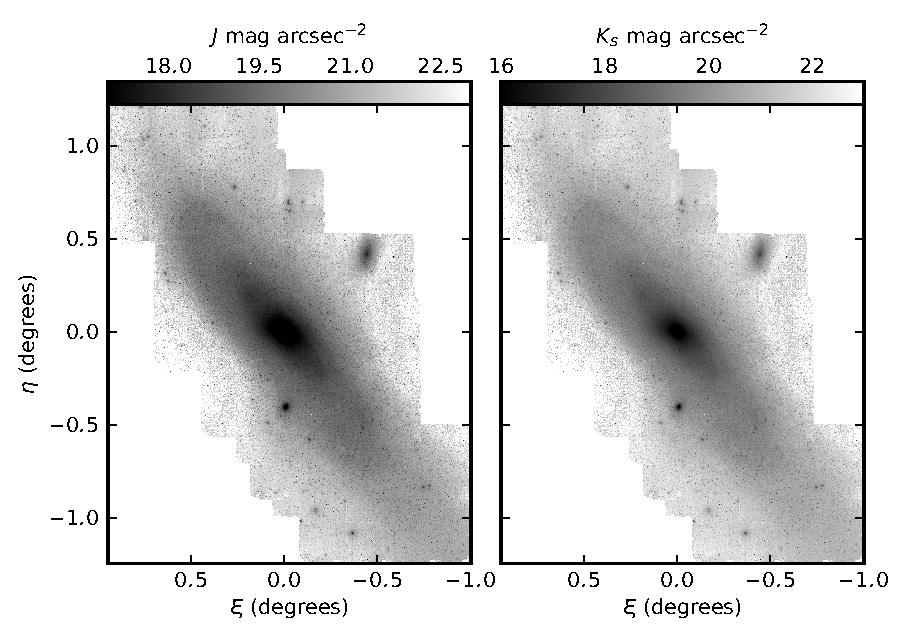
\includegraphics[width=3.5in]{figs/montage_planar_mosaics}
\caption{Montage-generated $J$ and $K_s$ maps. Compare to the equivalent simplex maps, \Fig{scalar_mosaics}. Pixels with negative surface intensity, after sky offset correction, are masked with white.}
\label{fig:montage_planar_mosaics}
% make with skysubpub/mosaic_plots.py and skyoffset/montageoffsets.py
\end{figure}

\sw{Montage} is also capable of fitting planar sky offsets to images, which is a tempting solution to the field-to-field discontinuities that persist between scalar-offset blocks.
The result of planar fitting is shown in \Fig{montage_planar_mosaics}.
We see that planar sky offsets, in this case, do little to improve the mosaics, and indeed, have a dramatic effect on the systematic surface brightness of the mosaic (by more than 1~mag~arcsec$^{-2}$ in the $K_s$ band).
Since our uncertainty on the shape of individual frames (0.3\% of the background level across a WIRCam frame) is significant compared to the uncertainty in background level, fitting planar offsets to each WIRCam field introduces additional systematic error propagation compared to scalar sky offsets.
\textit{We thus recommend against using planar, or higher-order, sky offsets in wide-field WIRCam mosaics.}

\subsection{Comparison to Spitzer/IRAC Images}

\begin{figure}[t]
\centering
\includegraphics[width=\columnwidth]{figs/sbdiff/scalar_irac36_sbdiff}
\caption{Maps of $J-[3.6]$ and $K_s-[3.6]$ surface colour inferred from the simplex scalar-sky fitted WIRCam mosaics and Spitzer/IRAC 3.6~$\mu$m image \citep{Barmby:2006}.
Note that the IRAC map crops the \androids/WIRCam footprint.}
\label{fig:scalar_irac36_sbdiff}
\end{figure}

We also explore systematic uncertainties in our WIRCam mosaics with comparisons against well-calibrated images of M31.
A template for the NIR disk is the 3.6~$\mu$m Spitzer/IRAC map, presented in \cite{Barmby:2006}.
Note that although Spitzer data avoid background subtraction issues caused by the NIR sky, planar sky offsets were used by \citeauthor{Barmby:2006}, though presumably of a smaller magnitude than our WIRCam sky offsets.
In \Fig{scalar_irac36_sbdiff} we compare our simplex scalar-fitted mosaics against the 3.6~$\mu$m image.
Generally the $J-[3.6]$ and $K_s-[3.6]$ colors decrease with disk radius, but increase in the star-forming regions due to hot dust emission.
However both colour maps (coincidentally) become redder in the south western disk beyond the 10~kpc star forming ring.
We interpret this as a systematic over-subtraction of background in these regions on the order of $\gtrsim 1$ mag~arcsec$^{-2}$.
Evidently, our scalar sky offset mosaics are not systematically reliable beyond the bright disk of M31, toward $R>15$~kpc.

\subsection{Monte Carlo Analysis of Systematic Surface Brightness Uncertainties}
\label{sec:montecarlo}

\begin{figure}[t]
\centering
\includegraphics[width=\columnwidth]{figs/bootstrap_sb_rms}
\caption{Mosaic maps of bootstrap RMS surface brightness in $J$ (left) and $K_s$ (right).
White contours identify RMS levels of 0.05 (solid), 0.1 (dashed) and 0.2 (dash-dot) mag arcsec$^{-2}$.}
\label{fig:bootstrap_sb_rms}
% made with skyoffset/bootstrap.py BootstrapRMSPlot
\end{figure}

The difference images presented in the previous section illustrate how the surface brightness reconstructions of identical data can vary depending on the optimization algorithm.
Here we pose a slightly different question: how are reconstructions affected by the initial conditions of background errors?
That is, given the possible sets of background level biases affecting the blocks, what is the distribution of surface brightness reconstructions?
We answer this with a realistic Monte Carlo analysis.

A Monte Carlo (MC) realization is generated by perturbing the surface brightness of the corrected blocks with a background error drawn (with replacement) from the ensemble of block sky offsets observed in the original mosaic (\Fig{scalar_mosaics}).
Using the scalar-sky fitting procedure, sky offsets  are optimized against the known sky background perturbations; 100 such realizations are made to compile an ensemble of mosaics in both bands.

Figure~\ref{fig:bootstrap_sb_rms} shows the RMS deviation of MC mosaic surface brightness against the original scalar-fitted mosaics.
Reconstructed surface brightness in the outer disk can vary by $\sim 1$~mag~arcsec$^{-2}$, consistent with colour biases in the $J-[3.6]$ and $K_s-[3.6]$ maps.

We can ultimately understand the source of surface brightness by examining the standard deviations in the residual between expected and realized sky offsets in each Monte Carlo iteration.
This residual dispersion is 0.15\% of the $J$-background (0.17\% of the $K_s$ background); we find this dispersion to be constant across all fields in the mosaics.
If mosaic surface brightness uncertainty is caused by flexure in the mosaic---where blocks on the mosaic periphery are forced to conform to the surface brightness of more central and tightly coupled blocks---then outer blocks would have higher offset dispersion.
This is not the case.

Rather than mosaic flexure, a better model for \Fig{bootstrap_sb_rms} involves uncertainties in the \textit{post priori} adjustment for zero net offset (\Eq{netzero}).
Since block sky offsets have approximately Gaussian distributions with dispersions given in \Tab{offset_hierarchy}, the uncertainty in the net offset correction is simply $\sigma(\mathrm{block})/\sqrt{n_\mathrm{blocks}}$, where $n_\mathrm{blocks}=39$ in the combined 2007B and 2009B mosaic.
Given that $\sigma_{\Delta_B}\sim 1\%$, the expected uncertainty in the net offset correction is 0.16\%: in perfect correspondence to the observed mosaic uncertainty.
The dominant source of uncertainty shown in the MC simulations, \Fig{bootstrap_sb_rms}, is the use of an arithmetic mean of offsets to set an absolute zero-point, not flexure or uncertainty in the network of offsets.
This suggests that external zero-points could be very useful in replacing \Eq{netzero}.
Since no absolutely-calibrated NIR photometry of M31's surface brightness exists, we will discuss a method using panchromatic resolved stellar populations in a future work.

\section{Conclusions}
\label{sec:conclusions}

We have presented near-infrared ($J$ and $K_s$) images of M31's entire bulge and disk with CFHT/WIRCam.
These maps surpass the 2MASS \citep{Beaton:2007} and Spitzer \citep{Barmby:2006} mosaics with superior resolution that permits the identification of individual stars throughout M31's mid and outer disk.
The dataset is also complementary to the HST/WF3 PHAT survey \citep{Dalcanton:2012} by providing complete coverage of M31's disk within $R=22$~kpc, and by offering a broader NIR colour baseline ($J-K_s$) than is offered by WF3 (approximately $J-H$).
NIR mosaics of M31 have crucial applications for studies of the nearly attenuation-free stellar structure of our nearest spiral neighbour, and for tests of stellar population synthesis models in NIR regimes.

Our focus in this paper has been the establishment of procedures for accurately recovering the NIR surface brightness across 3~sq.~deg.\ of the M31 disk using a sky-target nodding observing strategy with WIRCam on CFHT\@.
We have compared two different observing methods to study the effects of sky target nodding cadences and patterns on sky subtraction uncertainties.
We have also developed and tested our WIRCam pipeline for flat fielding, zero-point estimation, median sky subtraction, and sky offset optimization.

We find that our NIR SB reconstruction is limited in two regimes: large scale reconstruction of surface brightness with sky offsets, and surface brightness \emph{shape} uncertainties across individual WIRCam images.
On a large scale, the necessity of nodding between sky and target limits our direct knowledge of the background level on the disk by $\gtrsim 2$\% of the background level.
Strictly minimizing latency between sky and disk integrations (as in the 2009B program) provides only limited improvement in our knowledge of the background level on the disk because of the overhead in nodding the telescope, and spatial structure in the NIR skyglow itself.
Sky offset optimization is successful in reducing block-to-block surface brightness differences to $<0.1$\% of the background level.
Given a realized set of blocks, our optimization algorithm reliably finds a consistent solution, so any errors in surface brightness shape across the mosaic are caused by errors in the shapes of individual blocks (see below).
There is, however, an uncertainty in our net zero offset, of order $\sim \sigma_{\Delta_B} / \sqrt{N_\mathrm{blocks}}$; 0.16\% of the background level.
This zero-point can ultimately be established using resolved stellar populations, the subject of a forthcoming \androids\ study.

The shape of a WIRCam frame can be affected by both flat field uncertainties and additive background uncertainties.
We recommend using sky flats built from images collected every night to calibrate WIRCam images since these capture the gain structure of WIRCam detectors (unlike dome flats).
We also tested sky flats built on longer time spans (across a WIRCam queue run) or shorter (updated every half hour), but find that these either introduce flat fielding biases or become responsive only to changes in additive background contamination, respectively.
Although an additive background (\eg thermal or scattered light) contaminates these flats, the influence of flat fielding errors on surface brightness shapes is minimal across the background-dominated mosaic.
Instead, we find that the surface brightness across WIRCam frames is uncertain by 0.3\% of the background intensity due to variations in the background between sky and target fields.

% We now summarize our analysis of the data taking and reduction methods developed in this work, and in doing so, formulate a set of best practices for similar wide-field NIR surveys employing sky-target nodding.

% \subsection{Recommendations for Conducting a Wide-field NIR Survey with Sky-Target Nodding}

% We first recommend that the sky-target nodding cadence be set to effectively build real-time sky flats, rather than simply track background level evolution.
% Such a program would involve sufficient sky frames to build a sky flat within a window of 20--30 minutes, where the sky is observed in several epochs at different locations in a sampling ring to minimize biases.

% In the $K_s$ band this objective is efficiently achieved, since the mean background flux on a WIRCam pixel is $450 \pm 80$ ADU~$\mathrm{s^{-1}}$.
% Given $T_\mathrm{exp}=25$~s, a $\mathrm{[S^3T^6]^3}$ program yields the necessary 9 sky integrations within 20~minutes and a maximum sky-target latency of 2~minutes.
% Each sky flat would be built from observations at three sites along the sky ring.

% Lower background flux in the $J$ band ($120 \pm 30$~ADU~s$^{-1}$) requires additional sky integration to achieve comparable sky flat $S/N$ as the $K_s$ band.
% Given $T_\mathrm{exp}=45$~s, a $\mathrm{[S^4T^4]^5}$ program yields the necessary 20 sky integrations in $\sim 40$ minutes, with a maximum sky-target latency of 2.2~minutes.

% Sky offset optimization is aided by having more independent blocks covering the target, since our net zero offset assertion is uncertain by $\sigma_{\Delta_B} / \sqrt{N_\mathrm{blocks}}$.
% Given that $\sigma_B$ cannot be reduced, increasing the number of \emph{independent} blocks (observed hours or even a night apart to decouple sky and instrumental biases) is the most reliable way to establish the absolute surface brightness accuracy of the mosaic.
% Since sky offsets are further biased by any shape errors in blocks (realized as our inability to diminish block-to-block offsets below $\sim 0.1\%$ of background brightness), we propose that blocks be interlaced by 50\% (so that one detector completely overlaps a detector from an adjacent blocks).
% This interlacing pattern would thus enable the marginalization of shape errors across the entire detector frame.
% By doubling the number of blocks, each with individually halved exposure times, the mosaic could be reproduced with an equivalent net integration time.
% % \todo{Would this scheme increase the uncertainty in the sky level of each block, since there would be only half as many blocks? Then again, we double the number of blocks, so the uncertainty should be unchanged. Verify this.}

\bigskip We thank Loic Albert and Karun Thanjavur, previously from CFHT, for their help with WIRCam I'iwi data products and procedures and the CFHT staff for many informative discussions and their diligence in performing the queue service observations. We are grateful for the Spitzer 3.6~$\mu$m mapping provided by Pauline Barmby (University of Western Ontario).
J.S. and S.C. acknowledge support through respective Graduate Scholarship and Discovery grants from the Natural Sciences and Engineering Research Council of Canada.
M.M is supported by NASA through a Hubble Fellowship grant HST-HF51308.01-A awarded by the Space Telescope Science Institute, which is operated by the Association of Universities for Research in Astronomy, Inc., for NASA, under contract NAS 5-26555.
This publication makes use of data products from the Two Micron All Sky Survey, which is a joint project of the University of Massachusetts and the Infrared Processing and Analysis Center/California Institute of Technology, funded by the National Aeronautics and Space Administration and the National Science Foundation.
This work is based on observations obtained with WIRCam, a joint project of CFHT, Taiwan, Korea, Canada, France, at the Canada-France-Hawaii Telescope (CFHT) which is operated by the National Research Council (NRC) of Canada, the Institute National des Sciences de l'Univers of the Centre National de la Recherche Scientifique of France, and the University of Hawaii. 
{\it Facilities:} \facility{CFHT (WIRCam)}, \facility{FLWO:2MASS}.

\bibliography{master}

\end{document}
